\documentclass[12pt]{article}
\usepackage{amsmath}
\usepackage{epsfig,psfrag}
\usepackage{natbib}
\usepackage{graphicx}
\usepackage[shortlabels]{enumitem}
\setlength{\textwidth}{6.5in}
\setlength{\textheight}{8.9in}
\setlength{\voffset}{-1in}
\setlength{\oddsidemargin}{0in}
\setlength{\evensidemargin}{0in}

%biblography of JFM Style
\bibliographystyle{jfm}

%Some mathematical Definitions
\def\o{\over}
\def\p{\partial}
\def\be{\begin{eqnarray}}
\def\ee{\end{eqnarray}}
\def\bes{\begin{subeqnarray}}
\def\ees{\end{subeqnarray}}

\def\f{\frac}
\def\lp{\left(}
\def\rp{\right)}
\def\lb{\left[}
\def\rb{\right]}
\def\lcb{\left\{}
\def\rcb{\right\}}
\def\n{\nabla}
\def\lap{\nabla^2}
\def\z{\zeta}
\def\ep{\epsilon}
\def\l{\lambda}
\def\befi{\begin{figure}}
\def\eefi{\end{figure}}
\def\a{\alpha}
\def\no{\noindent}
\def\h{\hat{}}
\def\bce{\begin{center}}
\def\ece{\end{center}}



\def\d{\text{d}}
\def\vep{\varepsilon}
\def\ep{\epsilon}
\def\la{\langle}
\def\ra{\rangle}
\def\th{\theta}
\usepackage{tikz}
\usepackage{circuitikz}
\usepackage{float}
\usepackage{hyperref}
\newcommand{\AZ}[1]{{\color{red}{Ahmad: #1}}}
\newcommand{\red}[1]{{\color{red}{#1}}}
\title{Porous Media Project}
\author{Ahmad}
\date{}

\begin{document}
\maketitle

\tableofcontents


\section{Introduction}
%
In order to study the porous media, we introduce a model that captures
flow behavior through a porous material. We consider the porous media
as a network of pores that are connected together through
connections. The schematic of our model is shown in
Fig. \ref{porous-schematic}. We use a random resistor networks on a
structured grid as our model to study the flow behavior. Each node
represents a pore and each edge represents the throats between
pores. We use simple Poiseuille flow through pipes to model fluid flow
through pipes. In each pipe with diameter $d$, length $L$, and pressure difference
of $\Delta P$ on both sides, results in a flow $Q$, where
%
\begin{align}
    \frac{\Delta P}{L}  = \frac{128}{\pi} \frac{\mu Q}{d^4} 
\end{align}
%
where $\mu$ is the viscosity of the fluid. The above relation is known
as Darcy's law. 

%
\begin{figure}[h]
  \centering
  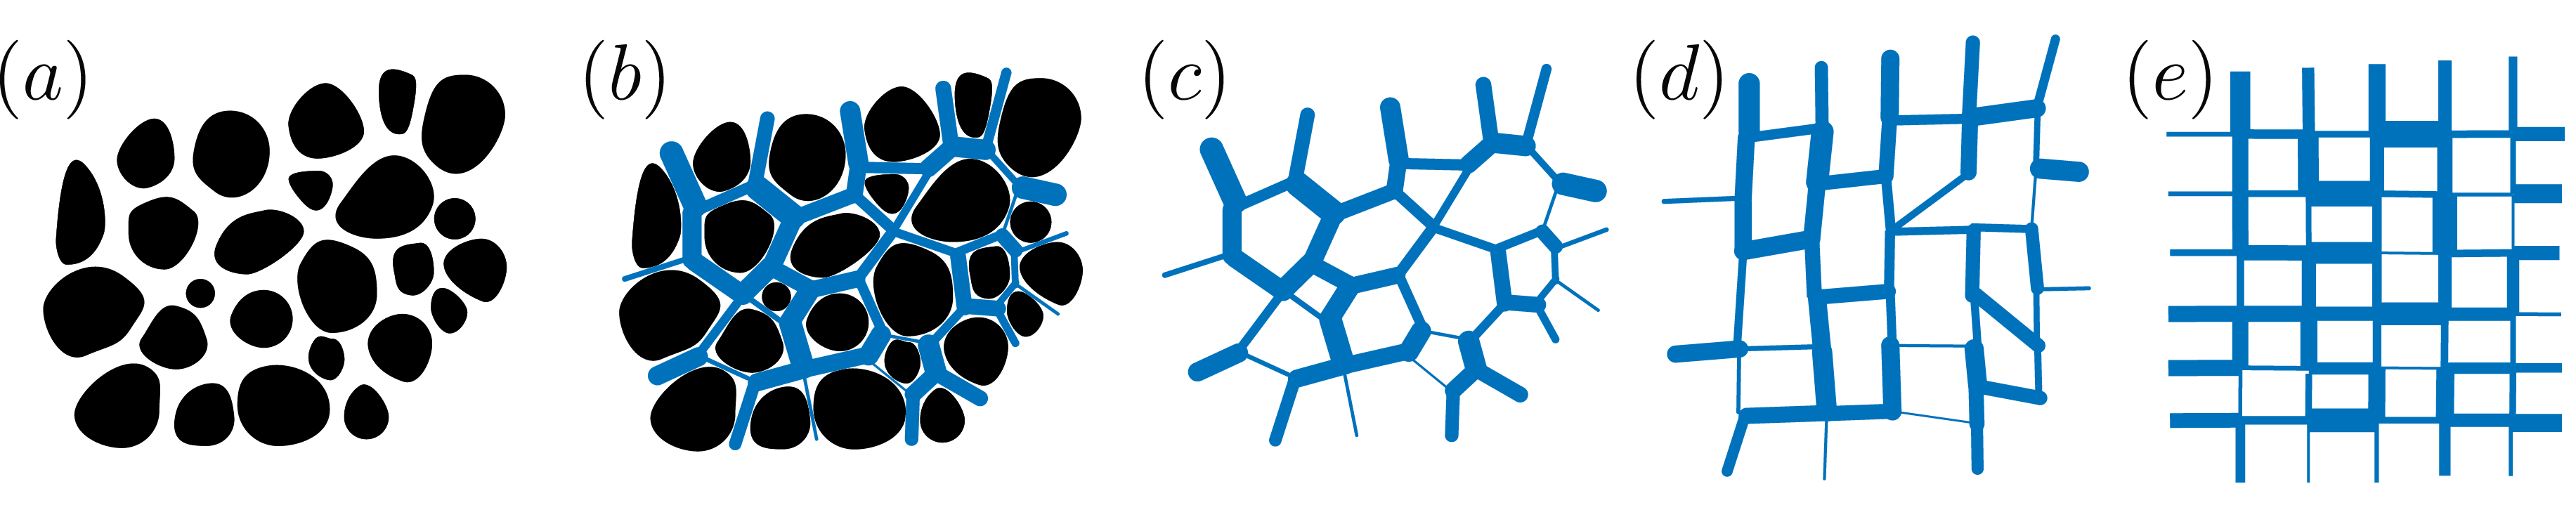
\includegraphics[width=\textwidth]{./Figs/porous-schematic}
  \caption{Schematic of the network model for porous media: (a) a
    sample cross section of a porous media. (b) The porous media can
    be considered as a network of pores connected through resistive
    connections. (c) The random network obtained from porous
    media. (d) Reordering the porous media network on a structured
    grid. (e) The ordered structured network used where the
    connections are assumed to be random resistors.} \label{porous-schematic}
\end{figure}
%

\section{Numerical Simulation}
%
We consider a network of tubes with a random distribution of diameters
as shown in Fig. {porous-schematic}e. Darcy's law is obtained thought
the momentum equation and relates the pressure and the flow through
the pipes. Furthermore, at each node the summation of the inflows
should add up to zero (conservation of mass). Using this a system of
equations $AP=B$ is obtained where $P$ is the vector of pressures at
nodes, $A$ is sparse where the nonzero elements are
% 
\begin{align}
  A_{ii} &= \sum_{j \text{ neighbors of } i} \frac{\pi }{128 \mu L} d_{ij}^4 \\
   A_{ij} &= 
  \begin{cases}
    -\frac{\pi }{128 \mu L} d_{ij}^4, \quad \text{if }j \text{ is
      neighbor of }i\\
    0, \quad \text{otherwise}
  \end{cases}
\end{align}
%
Note that if all the pipes have the same diameter, then the flow is
only in the horizontal pipes, and vertical pipes will carry no flow.


\subsection*{Numerical results}
%
We consider a 2d network of pipes, and a pressure difference between
the left and right nodes. We further assume different distribution of
pipe diameters and find the flow $q$ in the pipes. When the pipes are
all the same diameter, then the velocities in the pipes are either $0$
or some nonzero value. As we increase the randomness in the pipes, we
observe that the PDF of velocities starts to follow an exponential
tail trend. Interestingly, if the disorder in pipes diameter is large
enough, the PDF of velocities in the pipes, no matter what
distribution we pick follows the same distribution. 
%
\begin{figure}[h]
  \centering
  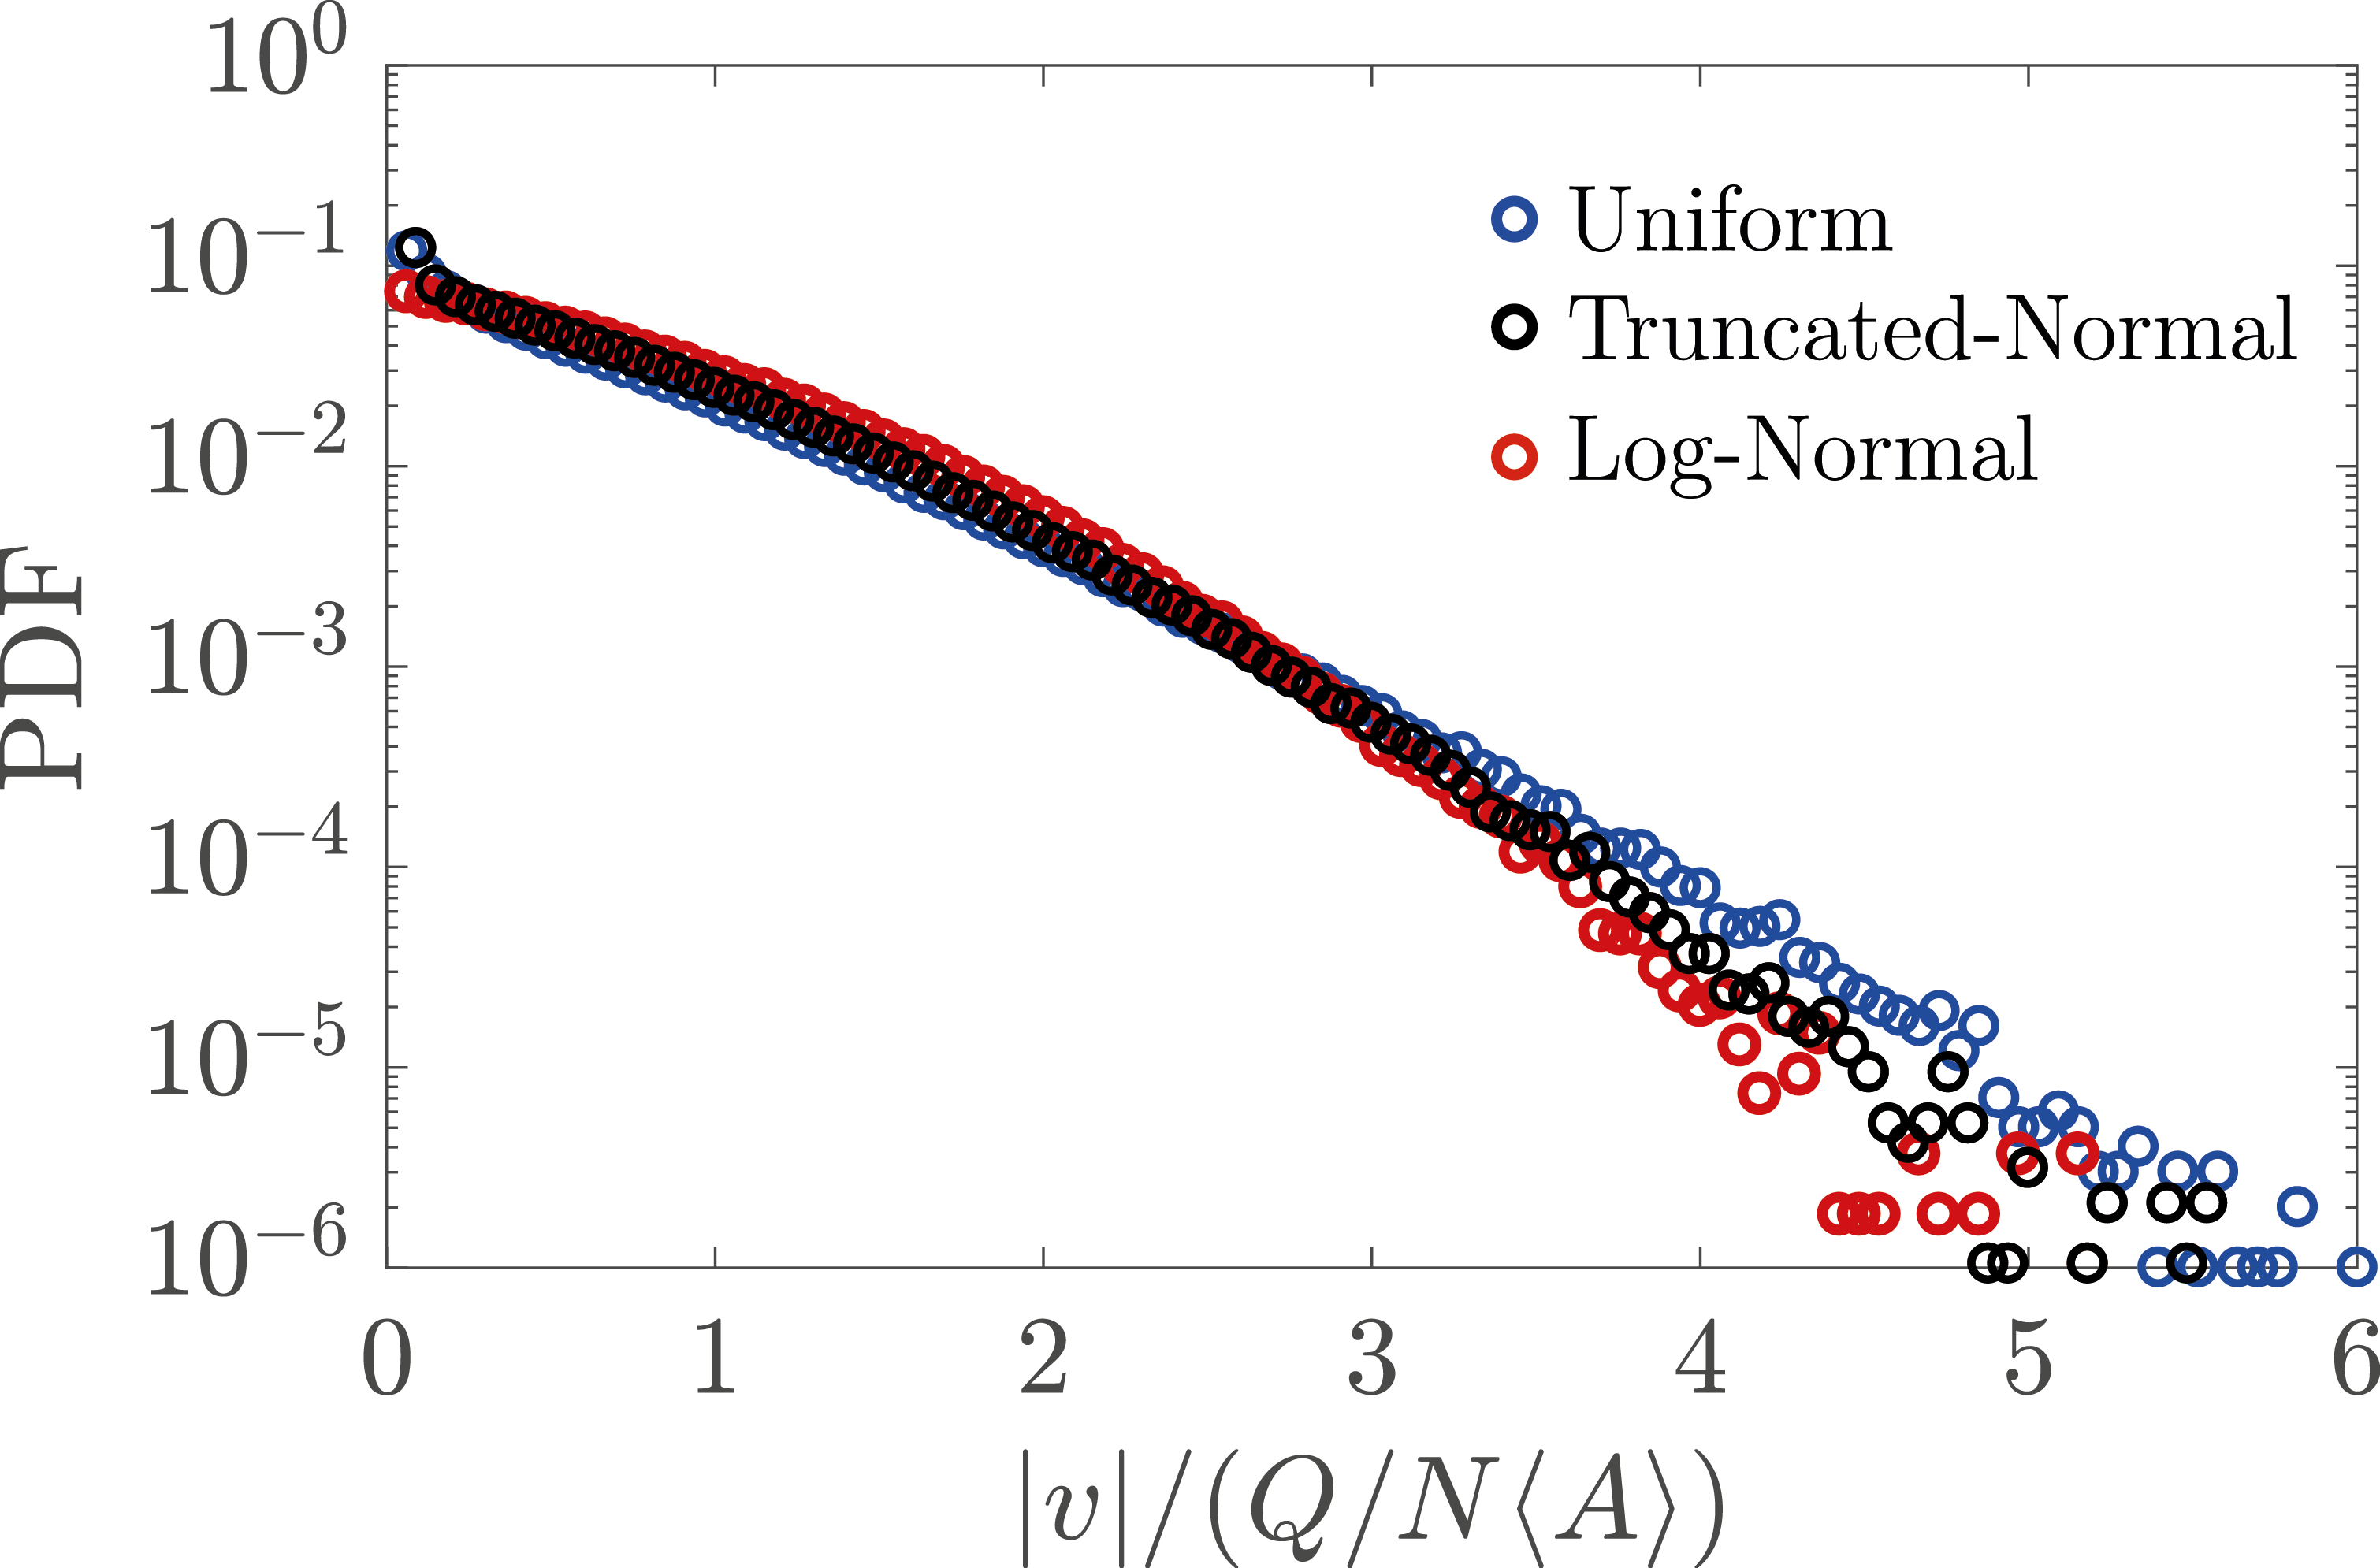
\includegraphics[width=0.6\textwidth]{./Figs/distribution}
  \caption{PDF of normalized velocities of the pipes in a random
    network of pipes, $v$ is the velocity in the pipe, $Q$ is the
    total flux, $N$ is the number of pipes in the vertical direction,
    $\langle A\rangle$ is the average of the area of the pipe. Note that
    $N\langle A\rangle$ is the average area carrying the flow $Q$. } \label{pdf-result}
\end{figure}


\section{Analytical results}
%
\label{sec:analytical}
In order to describe the universality observed above, we introduce the
following mode. First, instead of using the structured rectangular
grid, we use a structured diagonal grid. This will simplify the
analytical model (see Fig. \ref{grid-result}). 

%
\begin{figure}[h]
  \centering
  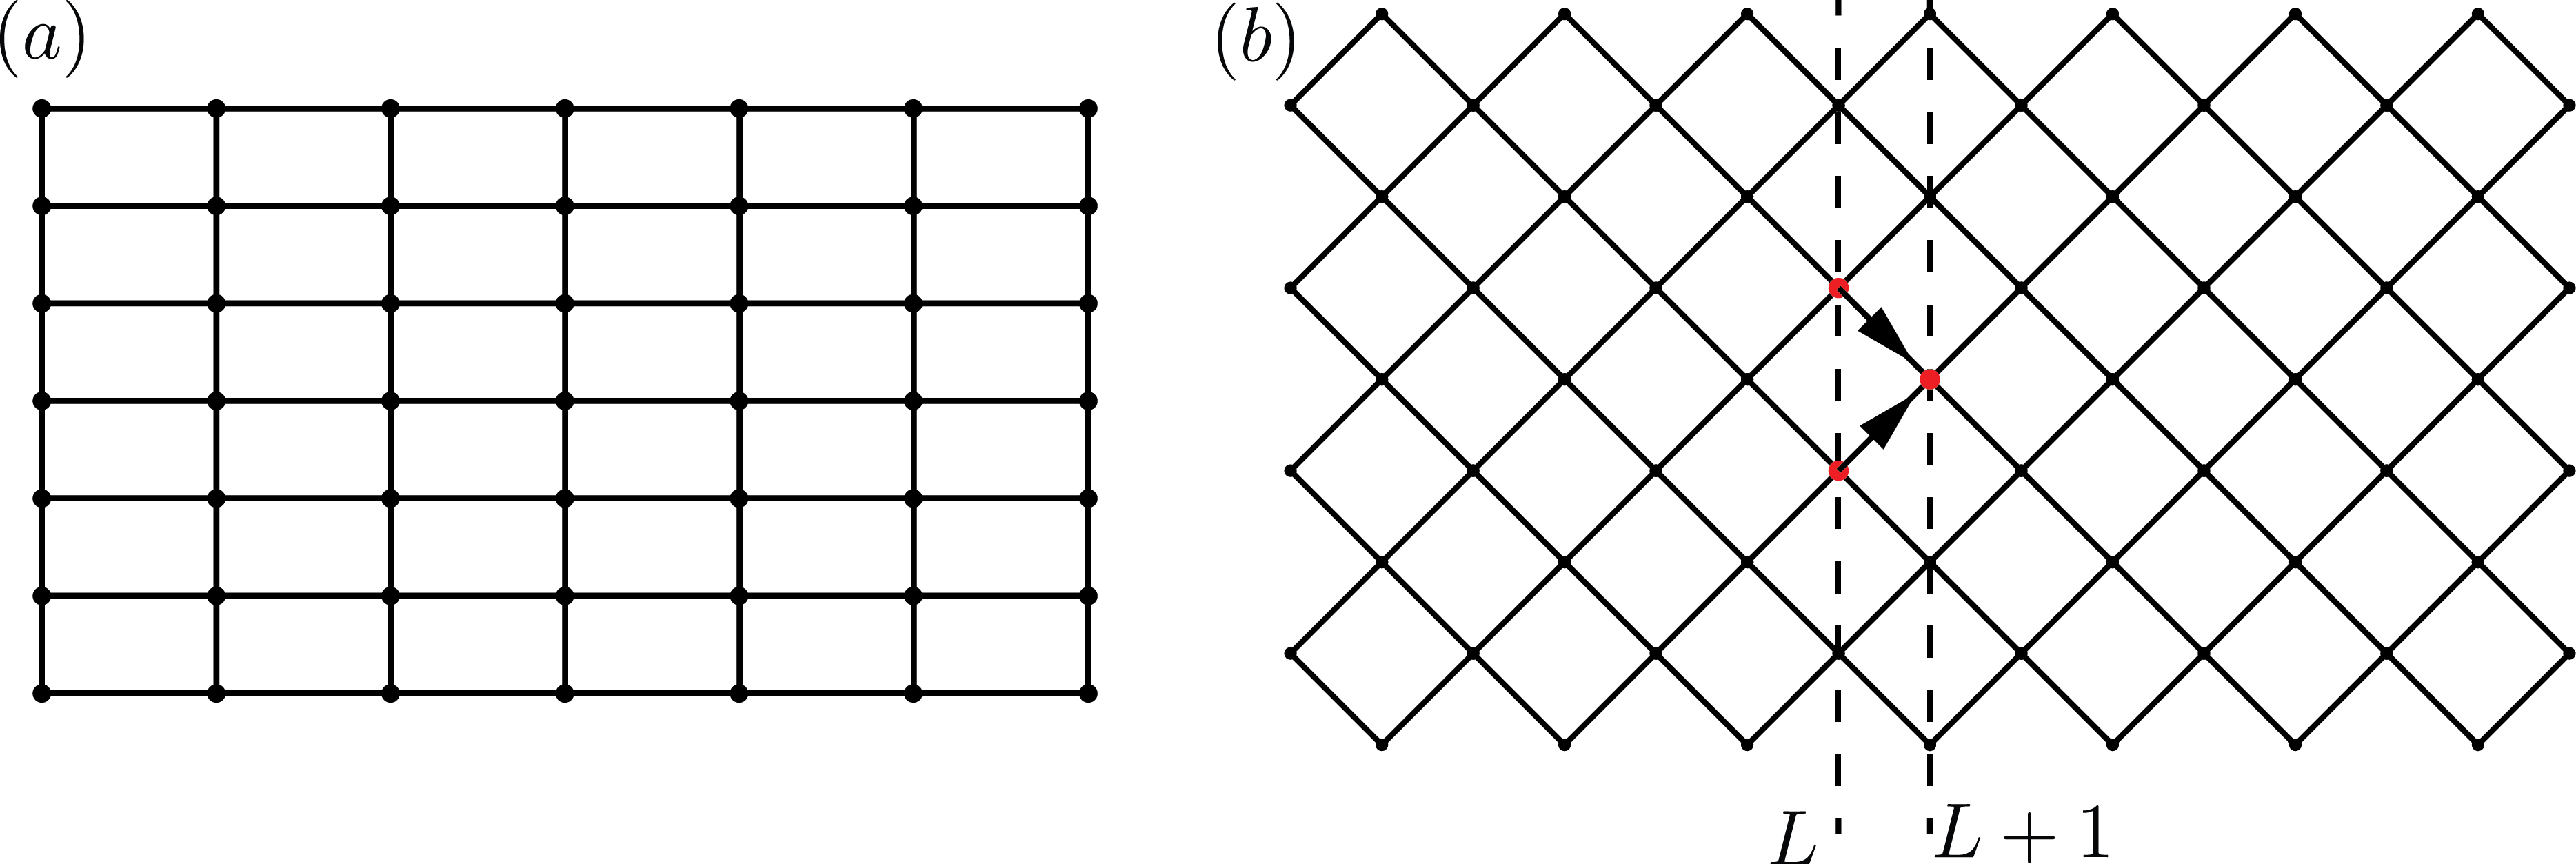
\includegraphics[width=1.0\textwidth]{./Figs/grid-analytica}
  \caption{Schematic of grids: (a) The structured rectangular grid
    used in the numerical simulation. (b) The structured diagonal grid
    used in the analytical model. } \label{grid-result}
\end{figure}
%
We assume that the total flow to node $i$ at level $L$ is noted by
$Q(L,i)$. This flow is then redistributed to the neighboring nodes at
the level $L+1$. We assume that this redistribution is done by weights
$w_{ij}$ as
%
\begin{align}
  Q(L+1,j) = \sum_i w_{ij} Q(L,i) = w_{i,i+1} Q(L,i+1) + w_{i,i} Q(L,i) \label{total-flow}
\end{align}
%
where $\sum_{j} w_{ij} = 1$ (since the total outflow from node $i$ is
$\sum_j q_iw_{ij}$ and this value should add up to $q_i$). We assume
that $w_{ij}$ are drawn from a distribution $\eta(w)$. Since $\eta(w)$
is a distribution, then $\int \eta(w) dw = 1$. Furthermore, since
$\sum_jw_{ij} = 1$, we can conclude that
%
\begin{align}
  \sum_j w_{ij}=1 \to N {E}[w_{ij}] = 1 \to E[w_{ij}] = 1/N \to {\int w\eta(w) dw = 1/N}
\end{align}
%

Now we use the technique of mean field analysis for a general
distribution of $\eta(w)$ to find the distribution of $Q$ at the
layers. The values of $Q(D,i)$ are not independent for neighboring
sites; however, the mean field approximation ignores these
correlations. We have
%
\begin{align}
  P_L (Q) = \prod_{j=1}^N \left\{ \int_0^1 d w_j \eta(w_j) \int_0^{\infty} dQ_j P_{L-1}(Q_j)\right\} \times \delta \lp \sum_j w_j Q_{j} - Q \rp
\end{align}
%
The constraint that $Q$'s emanating downward should add up to one is
in the definition of $\eta(w)$. The only approximation in the above
equation is that we neglect the possible correlation between the
values of $Q$ among ancestors. If we take the Laplace transform of
the above equation, we obtain
%
\begin{align}
  \tilde P(s) & \equiv \int_0^{\infty} P(Q) e^{-Qs} dQ\\
  \xrightarrow{\int_0^{\infty} (\cdot) e^{-Qs} dQ}  P (Q) & = \prod_{j=1}^N \left\{ \int_0^1 d w_j \eta(w_j) \int_0^{\infty} dQ_j P(Q_j)\right\} \times \delta \lp \sum_j w_j Q_{j} - Q \rp \\
  \tilde P(s) & = \int_0^{\infty} \prod_{j=1}^N \left\{ \int_0^1 d w_j \eta(w_j) \int_0^{\infty} dQ_j P(Q_j)\right\} \times \delta \lp \sum_j w_j Q_{j} - Q \rp e^{-Qs}dQ \\
              & = \prod_{j=1}^N \left\{ \int_0^1 d w_j \eta(w_j) \int_0^{\infty} dQ_j e^{-\sum w_{j}Q_{j}} P(Q_j)\right\}   \\
              & = \prod_{j=1}^N \left\{ \int_0^1 d w_j \eta(w_j) \tilde P(s w_j) \right\} \\
  & = \lp  \int_0^1 d w \eta(w) \tilde P(s w)  \rp^{N}
\end{align}
%
Or to summarize
%
\begin{align}
  \boxed{\tilde P(s) = \lp  \int_0^1 d w \eta(w) \tilde P(s w)  \rp^{N}} \label{eq:main-laplace}
\end{align}
%
Note that in the above equation $N$ determines the number of
neighboring sites and in our structured diamond grid $N=2$. The above
equation is recursively converges to a distribution.  If we set
$\eta(w) = \delta(w-1/2)$, then the flow at each node has probability of
$1/2$ to move up or down. As a result the flow at a given depth $L$
will be homogeneous as $P_L(Q) = \delta (Q-\bar{Q})$ where $\bar{Q}$
is the average of input fluid flow. This case is the same as the same
diameter which results in a singular solution in the structured grid.

\subsection*{$P(Q)$ decays faster than $Q^{-n}$ for any $n$}
We first show that $P(Q)$ decays faster than any power of $Q$ for any
weight distributions. We expand the Laplace transform as
%
\begin{align}
  \tilde P(s) = 1 + \sum_j \tilde P_{j} s^{j}
\end{align}
%
Inserting this expansion into Eq. \eqref{eq:main-laplace}, we obtain
%
\begin{align}
  1 + \sum_j \tilde P_{j} s^{j}  & = \lp  \int_0^1 d w \eta(w) \lb 1 + \sum_j \tilde P_{j} (sw)^{j}\rb    \rp^{N} \\
 & = \lp  1 + \sum_j \tilde P_j \langle w^{j}\rangle  s^{j}   \rp^{N}
\end{align}
%
where $\langle w^j \rangle = \int_0^1 \eta(w) w^j dw$ is the $j$-th
moment of the weights $w$. In the above equation we can observe that
%
\begin{align}
  P_j \lp N \langle w^j\rangle -1 \rp = G(P_{j-1}, P_{j-1}, \cdots, P_1)
\end{align}
%
In the above equation $P_j$ can only diverge only if $N\langle w^j
\rangle -1$ is zero. If $w$ can only be zero and one, then $\langle
w^j\rangle =\langle w \rangle = 1/N$ and the coefficient can become
zero! Other than this special distribution where $0 \leq w \leq 1$,
then
%
\begin{align}
  & w\in [0,1] \rightarrow w>w^2>w^3> \cdots \\
  & \forall k>1 \rightarrow \langle w^k \rangle < \langle w \rangle = \frac{1}{N} 
\end{align}
%
which means that $N\langle w^j \rangle -1$ is not zero and as a result
$P_j$ is finite. $P_j$ on the other hand is the $j$-th moment or
$\langle Q^j\rangle$ and it is finite. If $P\approx Q^{-n}$, then the
$n$-th moment will not be finite i.e. $\langle Q^{n+1}\rangle =
P_{n+1}$ is not finite. We can then conclude that $P(Q)$ should go to
zero faster than any $Q^{-n}$ as $Q\to \infty$! In other words $d \log
P(Q) / d \log Q \to -\infty$ as $Q\to \infty$.  

\subsection*{Exponential Decay}
%
The main governing equation for a diamond grid is 
%
\begin{align}
  \tilde P(s) = \lp  \int_0^1 d w \eta(w) \tilde P(s w)  \rp^{2} 
\end{align}
%
In order to have an approximation for $\eta(w)$ we do the following:
At each node there are two nodes where the flux is distributed by
$w_1$ and $w_2$. Lets assume that $w_1$ is uniformly distributed
between $0$ and $1$. As a result $w_2 = 1-w_1$ (since conservation of
mass $w_1 + w_2 = 1$). Now $\eta(w)$ can be found as
%
\begin{align}
  & \eta(w) = M \int_0^1 dw_1 \delta(1-w_1-w) =  M, \\
  \text{since }& \int_0^1 \eta(w) dw = 1 \to M =1 \\
  & \eta (w) = 1
\end{align}
%
Just for completeness, if there are three connections ($N=3$), then we
have
%
\begin{align}
  \eta(w) & = M \int_0^1 dw_1 \int_0^1 dw_2 \delta(1-w_1-w_2 - w)\\
          & = M(1-w)  \to \int_0^1\eta(w) dw = 1 \to M = \frac{1}{2} \\
  & \eta(w) = \frac{1}{2} (1-w)
\end{align}
%
As a result the main equation simplifies to
%
\begin{align}
  \tilde P(s) = \lp  \int_0^1 d w  \tilde P(s w)  \rp^{2} 
\end{align}
%
In order to solve the above equation, we assume $\tilde V (s) =
\sqrt{\tilde{P}(s)}$.
%
\begin{align}
  \tilde{V}(s) & = \int_0^1 dw \tilde V (sw) = \int_0^s \frac{du}{s}  \tilde{V}^{2}(u) \\
  s\tilde{V}(s) & = \int_0^s du  \tilde{V}^2(u) \\
\end{align}
%
Taking the differentiation with respect to $s$ yields
%
\begin{align}
  \tilde{V}(s) + s \frac{d \tilde{V}(s)}{d s} = \tilde{V}^2(s) \\
  \frac{d \tilde{V}}{\tilde{V}^2-\tilde{V}} = \frac{ds}{s}  \\
  \log\lp \frac{1-\tilde{V}}{\tilde{V}} \rp  = \log(s)\\
  \tilde{V}(s) = \frac{1}{1+Cs} 
\end{align}
%
We set the mean to $1$ i.e.,
%
\begin{align}
  \int_0^{\infty} Q P(Q) dQ = 1 \to \frac{d\tilde{P}}{ds}|_{s=0}  = -1\\
  \frac{d \tilde{V}}{ds}  = \frac{1}{2 \sqrt{\tilde{P}(s)}} \frac{d \tilde{P}(s)}{d s}   \to \frac{d\tilde{V}(s)}{ds}|_{s=0} =\frac{-1}{2} \\
  \frac{d\tilde{V}(s)}{ds} = \frac{-C}{(1+Cs)^{2}}|_{s=0} = -C = \frac{-1}{2}  \to C=\frac{1}{2} 
\end{align}
%
As a result, we have
%
\begin{align}
  \tilde{P}(s) = \lp\frac{1}{1+s/2} \rp^2 \\
  P(Q) = 4Q e^{-2Q}
\end{align}
%
We can then show that for a uniform distribution of $w$'s, the PDF of
$Q$'s become an exponential tail. For other distribution of $w$'s, we
similarly find a similar trend. Actually, we should that the PDF of
$Q$ should decay faster than any power law for any distribution of
$w$. Note that the only parameter that determines the the PDF of the
flow is the average flux. This shows that why we observe the universal
behaviour for pdf.

%
%
%
%
%

\section{Continuous Limit}
%
In the previous section (\S \ref{sec:analytical}), we used a toy model
to describe the flow behavior. The main equation connecting the flow
at different layers was Eq. \eqref{total-flow}. In this section, we
are interested to see what a continuous limit of the above model will
be. Consider Eq. \eqref{total-flow} as
%
\begin{align}
  Q(i,j+1) = w_{i-1,j} Q(i-1,j) + w_{i+1,j} Q(i+1,j) 
\end{align}
%
where we had a constraint on the weights as 
%
\begin{align}
  w_{i-1,j} + w_{i+1,j} = 1
\end{align}
%
Now, lets assume that these weights are perturbations around the a
uniform distribution such that
%
\begin{align}
  w_{i\pm 1,j}= \frac{1}{2}( 1 \pm v_{i\pm 1,j})
\end{align}
%
with th above assumption, we find that
%
\begin{align}
  Q(i,j+1) & = \frac{1}{2} \left( 1 - v_{i- 1,j}\right) Q(i-1,j) + \frac{1}{2} \left( 1 + v_{i+ 1,j}\right) Q(i+1,j)  \\
  Q + L_y \frac{\p Q}{\p y } + L^2_y \frac{\p^{2}Q}{\p y^2}  & = \frac{1}{2} (1-v + L_x \frac{\p v}{\p x}  ) \left( Q - L_x \frac{\p Q}{\p x} +   \frac{1}{2} L_x^2 \frac{\p Q^2}{\p x^2}\right) \nonumber\\
 & \qquad   +\frac{1}{2}  (1+v + L_x \frac{\p v}{\p x} )\left( Q + L_x \frac{\p Q}{\p x} + \frac{1}{2}L_x^2 \frac{\p^2 Q}{\p x^2} \right)  \\
  L_y \frac{\p Q}{\p y } & = L_x v \frac{\p Q}{\p x} + L_x \frac{\p v}{\p x} Q + \frac{L^2_x}{2} \frac{\p^{2}Q}{\p x^2}  \\
  \frac{\p Q}{\p y}    & = \frac{L_{x}}{L_{y}} \frac{\p }{\p x} \left( v Q \right)  + \frac{L^2_x}{2L_y} \frac{\p^{2}Q}{\p x^2}  
\end{align}
%
Assuming that $L_x = L_y $ (similar length scales in both directions),
we find that
%
\begin{align}
\boxed{\frac{\p Q}{\p y}  = \frac{\p}{\p x} \left( v Q\right) + D \frac{\p^{2} Q}{\p x^2}  }
\end{align}
%
which is a convection-diffusion equation.  It seems that $y$ direction
(the direction where flow propagates into the porous medium) acts
similar to time. As the flow moves inward, the $Q$ diffuses in the $x$
direction, and convects with velocity $v$. 



\section{Network Evolution}
%
Any changes to the micro-structure in a porous medium, such as solute
retention during polymer flow (effectively" clogging" some pores in
the network), affects the pore-level flow and alters the bulk
behavior. In this section, we want to study the effect of such
evolution in the network. The radius of the pipes in the network, can
reduce (due to clogging) or increase (due to erosion). The rate of
such reduction (or increase) can depend on flux, or shear rate, or
velocity, or etc. We can simplify these models with all the models
with the following equation
%
\begin{align}
  \frac{dR}{dt}  \propto \pm \frac{Q}{R^{n}} 
\end{align}
%
where $n=0,2,3$ corresponds to proportionality with flow rate,
velocity, shear gradient respectively. The plus sign corresponds to
erosion, and the negative sign corresponds to the clogging. In order
to study the effect of the above equation in whole network, we first
study the effect in a two parallel/series case.

\subsection{Erosion}
%
In erosion the rate of change of radius reads as
%
\begin{align}
  \frac{d r}{dt} & = \alpha \frac{Q}{r^{n}} 
\end{align}
%
Here, note that each pipe with radius $R$ acts as a resistor, we have
Poissoulle flow equation that relates the flow $Q$ to pressure
difference $\Delta P$ as
%
\begin{align}
  Q & = \frac{-\pi r^{4}}{8\mu L}  \Delta P\\
  Q & = -C(r) \Delta P, \quad C (r) = \frac{\pi r^{4}}{8\mu L} = {\beta}{r^{4}} 
\end{align}


\subsubsection*{Two pipes in series}

We consider two pipes in series as shown in
Fig. \ref{figure:resistor-series-1}. We are interested to see what
happens two the resistors for different initial conditions? How does
the values of the resistors evolve? What happens to the pressure
distribution at the note in between?
%
\begin{figure}[h]
  \begin{center}
    \begin{circuitikz}\draw
      (0,0) node[anchor=east] {$P_{l}$} to [short,o-] (0.1,0)
       to[R=$1/C_{1}$,-*] (2,0)  node [anchor=north] {$P_m$}
       to[R=$1/C_2$] (4,0)
       to[short,-o] (4.1,0) node [anchor=west] {$P_r$}; % The resistor
    \end{circuitikz}
    \caption{Two resistors at series}\label{figure:resistor-series-1}
  \end{center}
\end{figure}
%

We first simulate the results numerically to see what happens. The
results are shown in Fig. \ref{toy-series}. As it can be seen, for any
initial conditions the pressure at the middle point, converges to
$(P_l + P_{r})/2$ which basically means that the flow is homogenized.
%
\begin{figure}[!h]
  \centerline{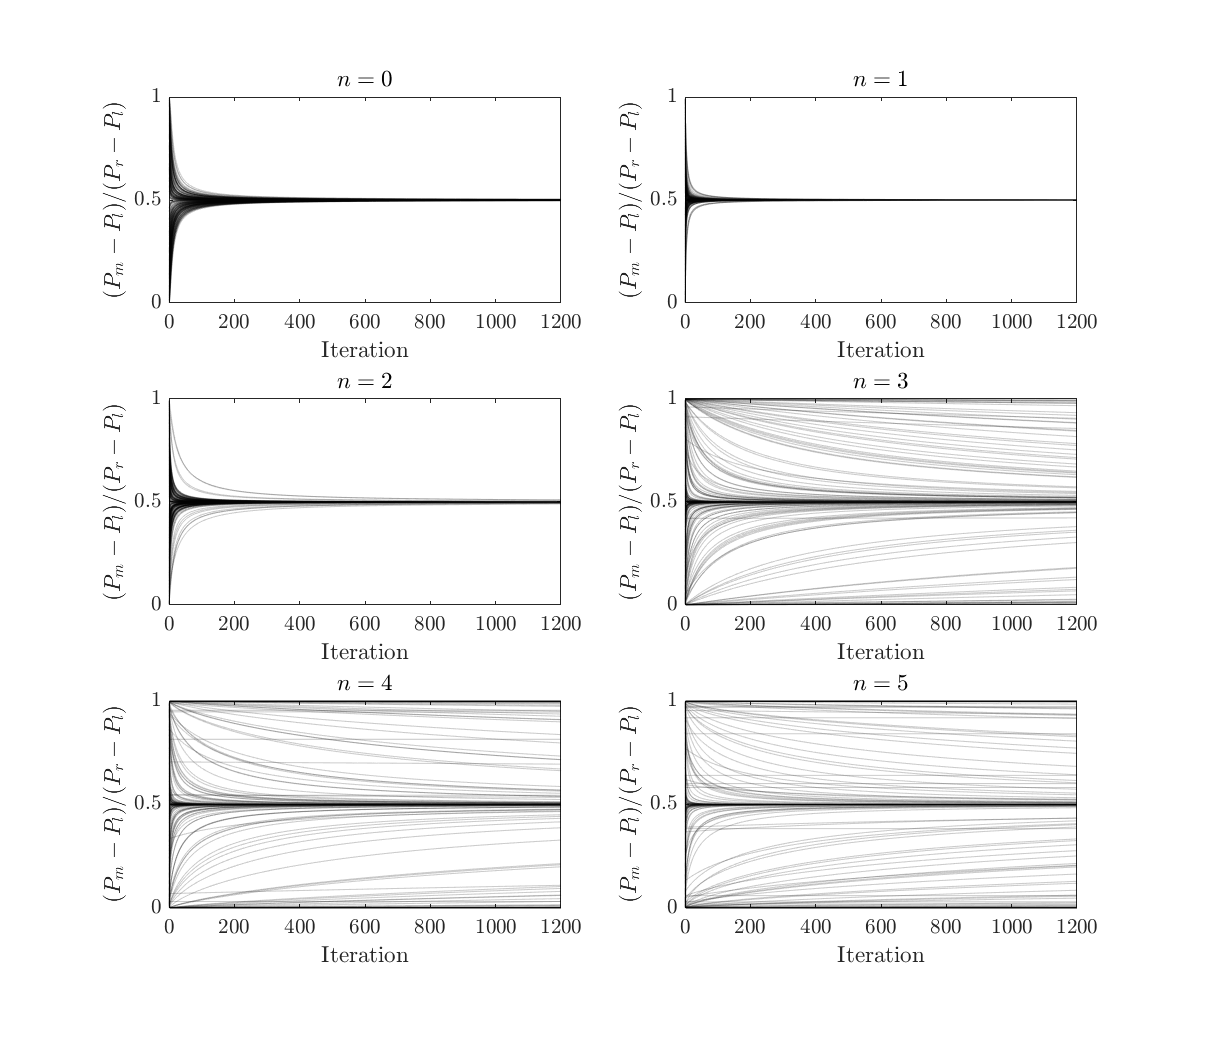
\includegraphics[width=1\textwidth]{./Figs/toy-model-series}}
\caption{Toy model for two pipes in series. In each iteration, we
  change the radius of the pipe as $r_{\text{new}} = r_{\text{old}} +
  \alpha Q/r_{\text{old}}^n$. For all different cases of $n$ the
  middle pressure converges to $(P_l + P_r)/2$.}
\label{toy-series}
\end{figure}  
%


We now show why this convergence happens. If the two pipes are in
series, then $Q$ is always the same in these two pipes. Therefore
%
%
\begin{align}
  \frac{d r}{dt} & = \alpha \frac{Q}{r^{n}} \\
  r^{n}{d r} & = \alpha {Q} dt \\
  \frac{1}{n+1} r^{n+1} -  \frac{1}{n+1} r_0^{n+1} & = \alpha Q t\\
  r & = \lp (n+1)\alpha Q t + r_0^{n+1}\rp ^{\frac{1}{n+1}} \\
  C_i & = \beta \lp (n+1)\alpha Q t + r_{i,0}^{n+1}\rp ^{\frac{4}{n+1}}
\end{align}
%
So the pressure at the middle point becomes as 
%
\begin{align}
  Q &= \frac{1}{1/C_{1} + 1/C_2}   \Delta P = \text{const.}, \\
  P_m - P_l &= \frac{Q}{C_{1}}   \\
  \frac{P_{m}-P_l}{P_r - P_l} & = \frac{1/C_{1}}{1/C_{1} + 1/C_2} = \frac{C_{2}}{C_{1} + C_2}  
\end{align}
%
Combining the results we find that
%
\begin{align}
  &\boxed{\frac{P_{m}-P_l}{P_r - P_l} = \frac{\beta \lp (n+1)\alpha Q t + r_{2,0}^{n+1}\rp ^{\frac{4}{n+1}}}{\beta \lp (n+1)\alpha Q t + r_{1,0}^{n+1}\rp ^{\frac{4}{n+1}} + \beta \lp (n+1)\alpha Q t + r_{2,0}^{n+1}\rp ^{\frac{4}{n+1}}} } \\
  &\lim_{t\to\infty} \frac{P_{m}-P_l}{P_r - P_l}  = \frac{1}{2} 
\end{align}
%
Note that for any power of $n$ the pressure in the middle point as $t\to\infty$
converges to $(P_l+P_r)/2$. 

\newpage
\subsubsection*{Two Parallel Pipes Case}
%
Now assume two pipes in parallel as shown in
Fig. \ref{figure:resistor-series-par}. We first simulate the results
to see what happens for different initial conditions. The results for
different initial values of $r_1,r_2$ are shown in Fig. \ref{toy-par}.
%
\begin{figure}[!h]
  \begin{center}
    \begin{circuitikz}
      \draw
      (-0.5,0) node[anchor=east] {$P_{l}$} to [short] (0.1,0)
      -- (0.1,0.5) 
       to[R=$1/C_1$] (2,0.5)  -- (2,0) to [short] (2.5,0) node
       [anchor=west] {$P_r$};
      \draw
      (0.1,0)  --(0.1,-0.5) 
       to[R=$1/C_2$] (2,-0.5)  -- (2,0);
    \end{circuitikz} 
    \caption{Two resistors parallel together} \label{figure:resistor-series-par}
  \end{center}
\end{figure}
%


\begin{figure}[!h]
  \centerline{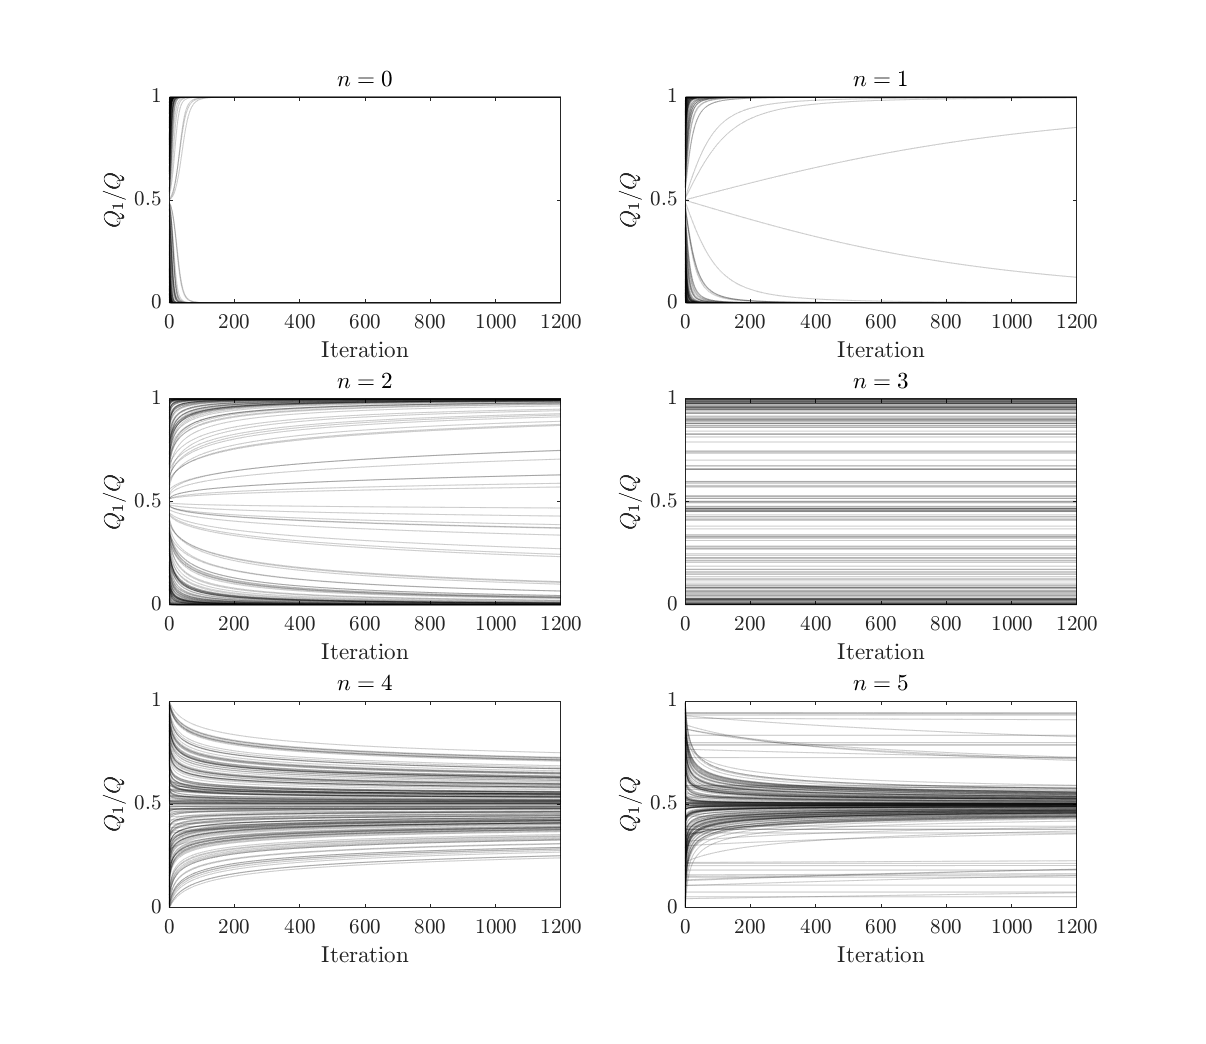
\includegraphics[width=1\textwidth]{./Figs/toy-model-par}}
  \caption{Toy model for two pipes in parallel. In each iteration, we
    change the radius of the pipe as
    $r_{\text{new}} = r_{\text{old}} + \alpha
    Q_{i}/r_{\text{old}}^n$. When $n<3$, all of the flow eventually
    passes from either top or bottom pipe. When $n=3$, the flow
    proportion remains the same. When $n>3$, the flow homogenizes
    where half of the total flow i.e. $Q/2$ passes from top and the
    other half from bottom pipe.}
\label{toy-par}
\end{figure}  

Now, we start to model to see why this happens. Initially, we note
that
%
\begin{align}
  Q_1 = C_1 \Delta P, \quad \text{ and }\quad Q_2 = C_2 \Delta P \\
  Q = (C_1 + C_2) \Delta P
\end{align}
%
We change the radius of each pipe according to its flow, as a result,
we have
%
\begin{align}
  \frac{dr_{1}}{dt}  = \alpha \frac{Q_{1}}{r_{1}^n}, \qquad  \frac{dr_{2}}{dt}  = \alpha \frac{Q_{2}}{r_{2}^n} \\
  r_1^n \frac{dr_{1}}{dt}  + r_2^n \frac{dr_{2}}{dt}  = \alpha (Q_1 + Q_2) = \alpha Q  
\end{align}
%
On the other hand, we know that
%
\begin{align}
  \Delta P = \frac{Q_{1}}{C_{1}}  = \frac{Q_{2}}{C_{2}} \\
  \Delta P = \frac{Q_{1}}{\beta r_1^{4}}  = \frac{Q_{2}}{\beta r_2^{4}}   \\
  \frac{dr_{i}}{dt}  = \alpha \frac{Q_{i}}{r^{n}_{i}} = \frac{\alpha \beta \Delta P}{r^{n-4}_{i}}   
\end{align}
%

We have
%
\begin{align}
  &r_{1}^{n-4} \frac{dr_{1}}{dt} = r_2^{n-4}\frac{dr_{2}}{dt}\\
  &\text{if }n=3, \quad \to \log(\frac{r_{1}}{r_{1,0}}) = \log(\frac{r_{2}}{r_{2,0}}), \to r_1 = \gamma r_2 \\
  & \text{if }n\neq 3, \quad r_1^{n-3} - r_2^{n-3} = \gamma
\end{align}
%
where $\gamma$ is a constant. In the above equation, without loss of
generality, we can assume that $r_{1}>r_2$ and $\gamma$ is
positive. Now, looking at the other part of the equation, we have
%
\begin{align}
  \frac{dr_{2}}{dt}  & =  \frac{\alpha \beta \Delta P}{r^{n-4}_{2}} \\
                     & = \frac{\alpha \beta }{r^{n-4}_{2}} \frac{Q}{\beta (r_{2}^{4} + r_1^4)} = \frac{\alpha Q}{r^{n}_{2} + r_{2}^{n-4} r_1^{4}} \\
                     & = \frac{\alpha Q}{r^{n}_{2} + r_{2}^{n-4} \lp r_2^{n-3} + \gamma \rp^{\frac{4}{n-3} }}\\
  \lb r^{n}_{2} + r_{2}^{n-4} \lp r_2^{n-3} + \gamma \rp^{\frac{4}{n-3} }\rb dr_2 & = \alpha Q dt\\
  \frac{1}{n+1} \lb r_2^{n+1} + \lp r_2^{n-3} + \gamma\rp^{\frac{n+1}{n-3} } \rb  & = \alpha Qt + C\\
  r_2^{n+1} + \lp r_2^{n-3} + \gamma\rp^{\frac{n+1}{n-3} }  & = (n+1)\lp \alpha Qt + C\rp \\
  r_2^{n+1} + r_{1}^{n+1} = At+B
\end{align}
%
So the two set of equations summarizes to
%
\begin{align}
  & \begin{cases}
    r_1^{n-3} - r_2^{n-3} = \gamma \quad \text{ if }n \neq 3,   \\
    r_1 = \gamma r_{2} \quad \text{ if } n=3
  \end{cases}\\
  & r_1^{n+1} + r_2^{n+1} = At + B
\end{align}
%
The plot for the solution to the above equations for different values
of $n\neq 3$ and also the separate solution for $n=3$ is shown in the
following figure.  
%

\begin{figure}[!h]
  \centerline{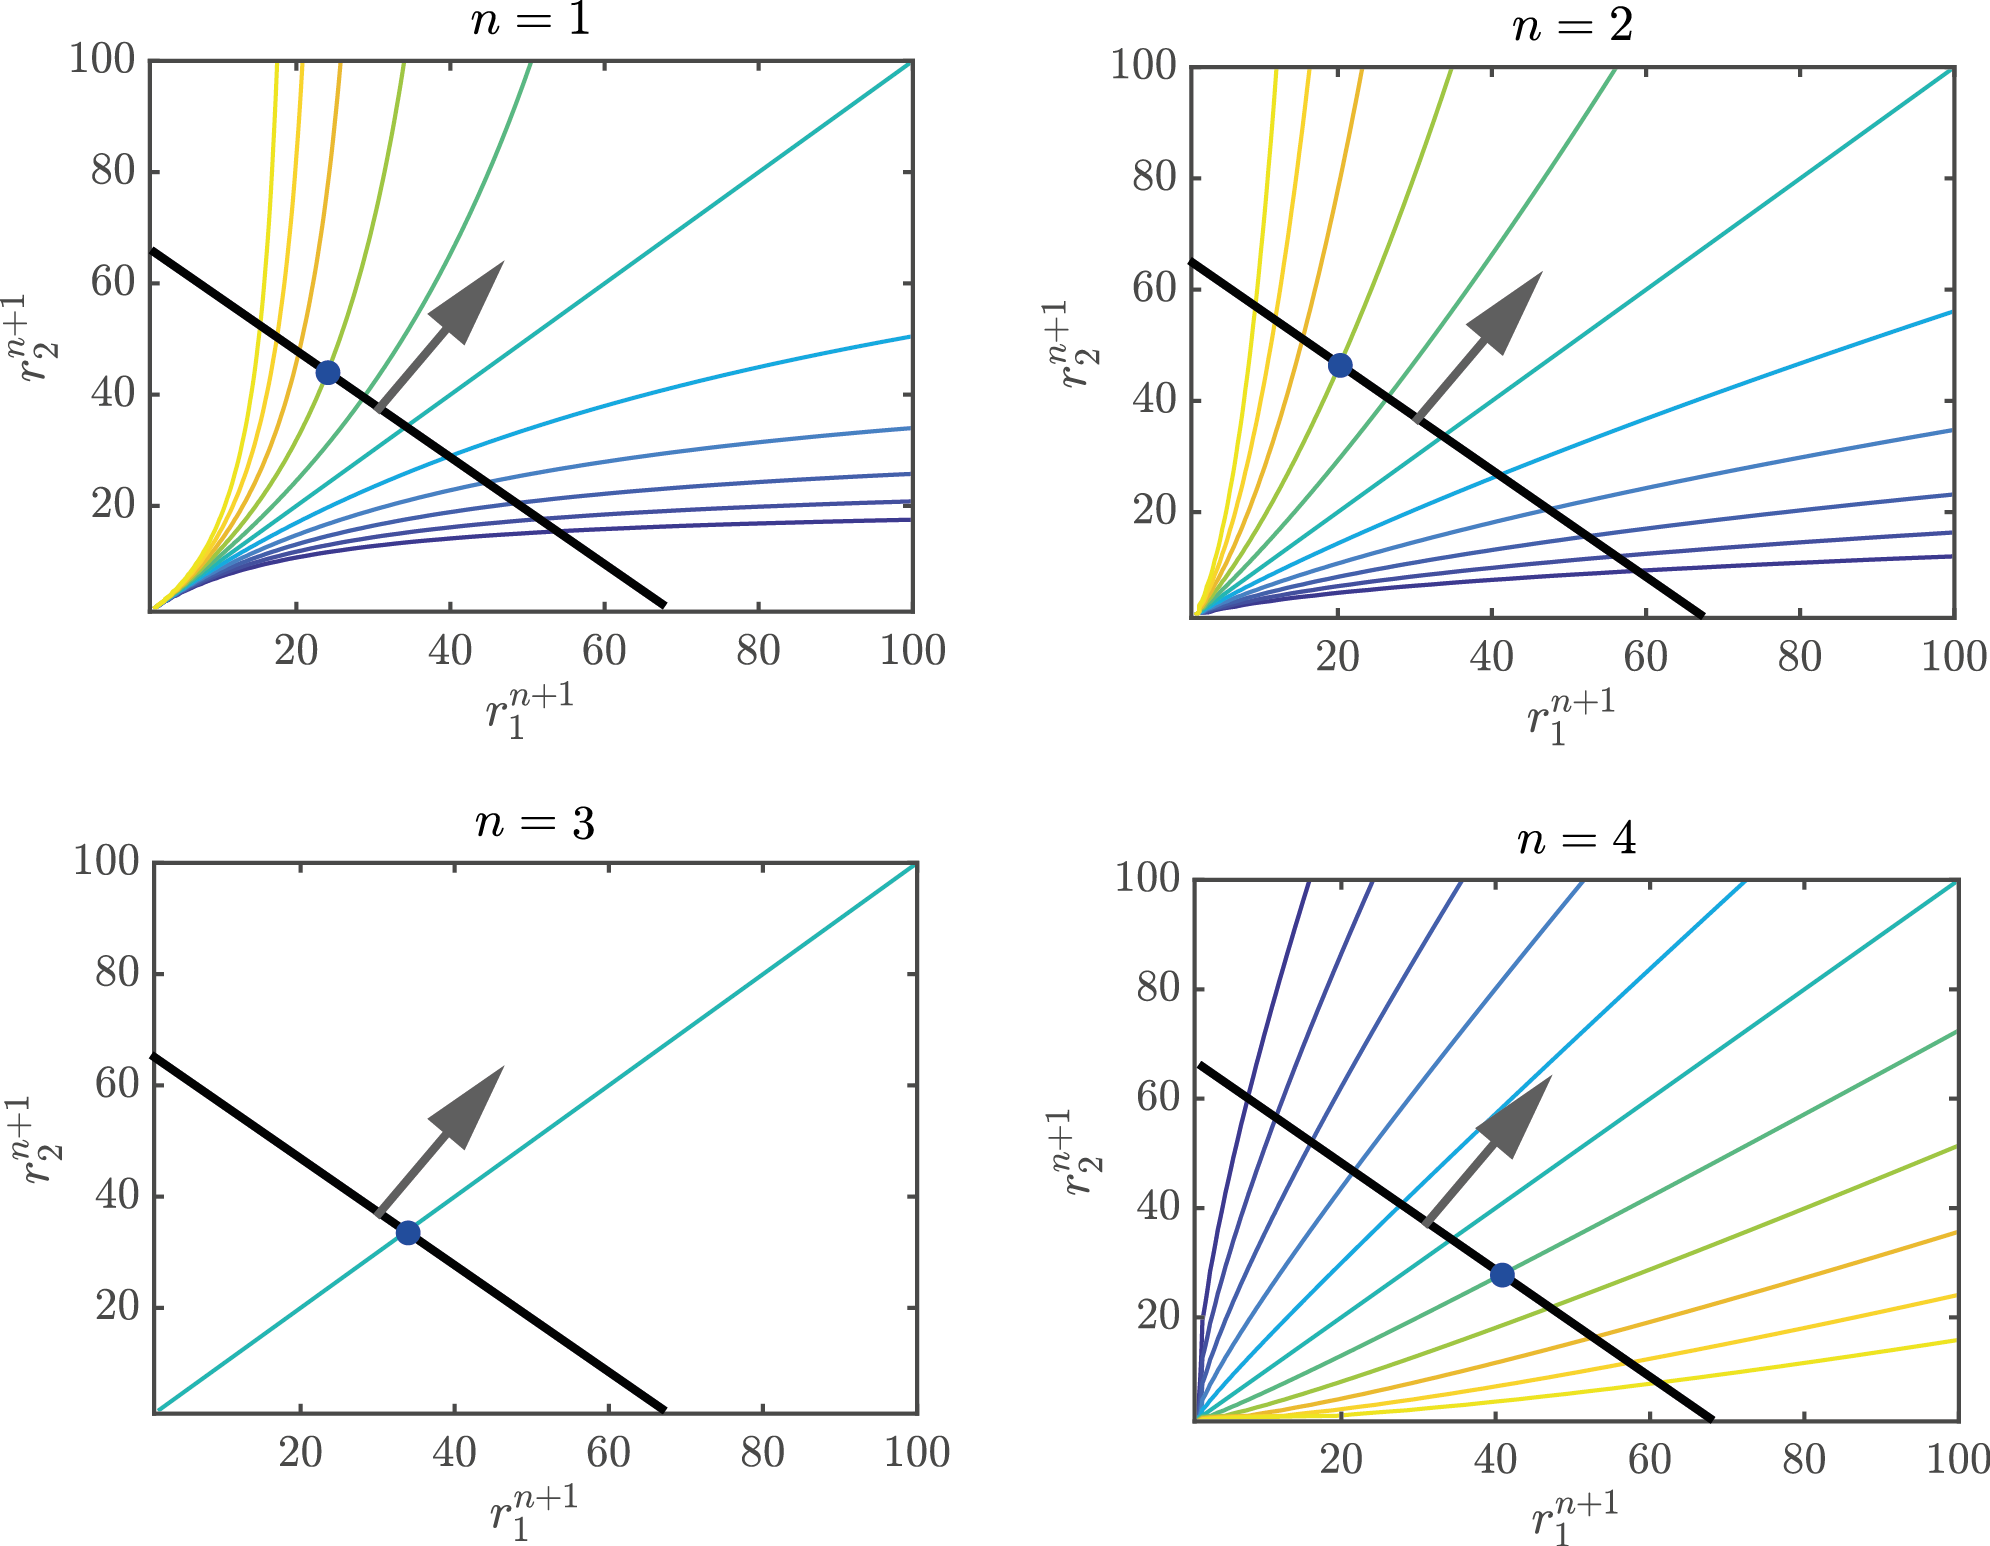
\includegraphics[width=0.8\textwidth]{./Figs/par_resistors}}
  \caption{Analytical solution for $r_1$ and $r_2$ for parallel
    resistors. For different $n$ the solution changes. Specifically,
    if $n<3$, then one of the diameters stops varying while the other
    one increases in size. If $n=3$, the both grow together, and if
    $n>3$ then they both increase in size. }
\label{anal-par}
\end{figure}  


\subsubsection*{General Case}
%
In a general case, the resistors can be divided into series and
parallel resistors. Using that in each section, we only need to look
at the parallel resistors and determine the channelling. The resistors
in series do not affect the channelling to occur. They only contribute
tot he homogenization. Parallel resistors however, in the case of
$n>3$ result in channeling. Note that at some places, we might need to
use $\Delta-Y$ conversion to find the equivalent resistors. It can be
shown that the channeling can still be described using $\Delta-Y$
conversion.


\subsubsection{Some Corrections to Series and Parallel cases(Deng)}
\AZ{The case example here is the special case where $C_2=C_3$ in the series part and also $C_\text{eq}=C1$ where $C_\text{eq}$ is the equivalent resistor resulted from $C_1$ and $C_2$. This special case always results in the same fluid flux in the resistors. This special case can also be observed from the diagonal contour line present in Fig. \ref{anal-par}. } Numerical simulations show different result here for more complex cases other than naive parallel or series cases. For example for the following case Fig \ref{resistor-par-series21}.
\begin{figure}[ht]
    \begin{center}
    \begin{circuitikz}
      \draw
      (-0.5,0) node[anchor=east] {$P_{l}$} to [short] (0.1,0)
      -- (0.1,0.5) 
       to[R=$1/C_1$] (2,0.5)  --  (4,0.5)  -- (4,0) to [short] (4.5,0) node
       [anchor=west] {$P_r$};
      \draw
      (0.1,0)  --(0.1,-0.5) 
       to[R=$1/C_2$] (2,-0.5) to[R=$1/C_{3}$] (4,-0.4)--(4,0);
    \end{circuitikz} 
    \caption{Parallel/Series Case (Deng)} \label{resistor-par-series21}
  \end{center}
  
\end{figure}
The simulations are similar to previous ones that keep the flow constant while increasing the radius proportional to $Q/r^n $. It now shows that the flow does not need to be homogeneous through top and bottom tubes. A special case can be easily analytically calculated. Set $C_{1}(t=0) = 2, C_{2}(t=0)=C_{3}(t=0) = 1$, and let $n=7$, in this case 
\begin{equation}
    \frac{dC_i}{dt} = 4Q_i/C_i
\end{equation}
and $C_2=C_3$ will always hold, and it is not difficult to solve $C_1$ and $C_2$
\begin{align}
    \frac{dC_1}{dt} = \frac{8Q}{C_2+2C_1} \\
    \frac{dC_2}{dt} = \frac{4Q}{C_2+2C_1},
\end{align}
where $Q$ is the total flow. In fact we do not need to solve these simple equations and it is clear that at the end we get $C_2=C_3=1/2 C_1$ since $\frac{dC_1}{dC_2} = 2$. However, this means at the end $Q_1/Q = 4/5$ instead of $1/2$. 

Intuitively, the failure of equalization of flow is due to the non-linearity of erosion law, which voids the common sense that two resistors in series can be combined as one. Therefore we expect the conclusions in this paper could be affected by the network structure.
\subsubsection{More general numerical results of Fig. \ref{resistor-par-series21}}
In general as we set $\frac{dr_i}{dt} = Q_i/r_i^n$ and $C_i = r_i^4$, in the network of Fig. \ref{resistor-par-series21} we have 
\begin{align}
    \frac{dC_1}{dt} &= \frac{4QC_1^{(7-n)/4}}{\Delta} \\
    \frac{dC_2}{dt} &= \frac{4QC_2^{(7-n)/4}C_3}{\Delta(C_2+C_3)} \\
    \frac{dC_3}{dt} &= \frac{4QC_3^{(7-n)/4}C_2}{\Delta(C_2+C_3)},
\end{align}
where $\Delta = C_1+\frac{C_2C_3}{C_2+C_3}$, the ratio $Q_1/Q_2 = C_1(C_2+C_3)/(C_2C_3)$. Fig. \ref{toy-par-series-eros} are the numerical result for $n=5$ and $n=7$ with $C_2(t=0)=C_3(t=0)=1$ and changing $C_1(t=0)$. $Q_1/Q_2$ are not converging to 1 in either case.  
\begin{figure}[H]
  \centerline{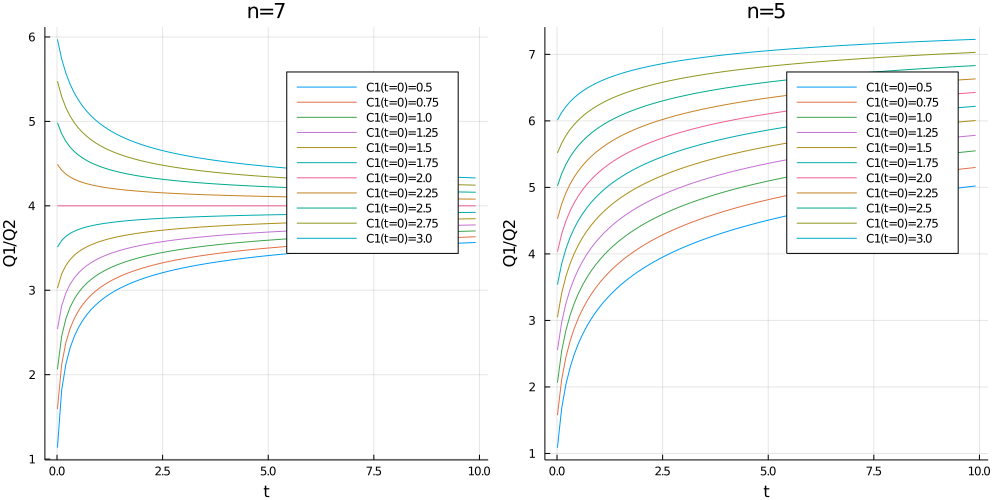
\includegraphics[width=1\textwidth]{Figs/par_series_12.png}}
  \caption{For different n and $C_1(t=0)$, the simple network under erosion yields different $Q_1/Q_2$.}
\label{toy-par-series-eros}
\end{figure}  
\newpage
\subsection{Clogging}
%
In clogging, the rate of change of radius reads as
%
\begin{align}
  \frac{dr}{dt } = -\alpha \frac{Q}{r^{n}} 
\end{align}
%
Similar to the erosion, we first study a simplified model with two
pipes in series and parallel.


\subsubsection*{Series}
%
We consider the following pattern for the resistors
(Fig. \ref{figure:resistor-series-clogging}). We first simulate for different initial conditions, and look at the
middle pressure over long time. Since the radius is decreasing, we
need to set a maximum amount of reduction. Since the radius cannot
become negative. For different initial conditions we look at the
middle pressure, and we observe that no matter what power of $n$ is,
the middle pressure remains almost unchanged. If the minimum threshold
is hit, then some jumps can be observed, however, the total behavior
is such that the ratio of the middle pressure remains almost similar.

%
\begin{figure}[!h]
  \begin{center}
    \begin{circuitikz}\draw
      (0,0) node[anchor=east] {$P_{l}$} to [short,o-] (0.1,0)
       to[R=$1/C_{1}$,-*] (2,0)  node [anchor=north] {$P_m$}
       to[R=$1/C_2$] (4,0)
       to[short,-o] (4.1,0) node [anchor=west] {$P_r$}; % The resistor
    \end{circuitikz}
    \caption{Two resistors at series}\label{figure:resistor-series-clogging}
  \end{center}
\end{figure}
%

% 
\begin{figure}[H]
  \centerline{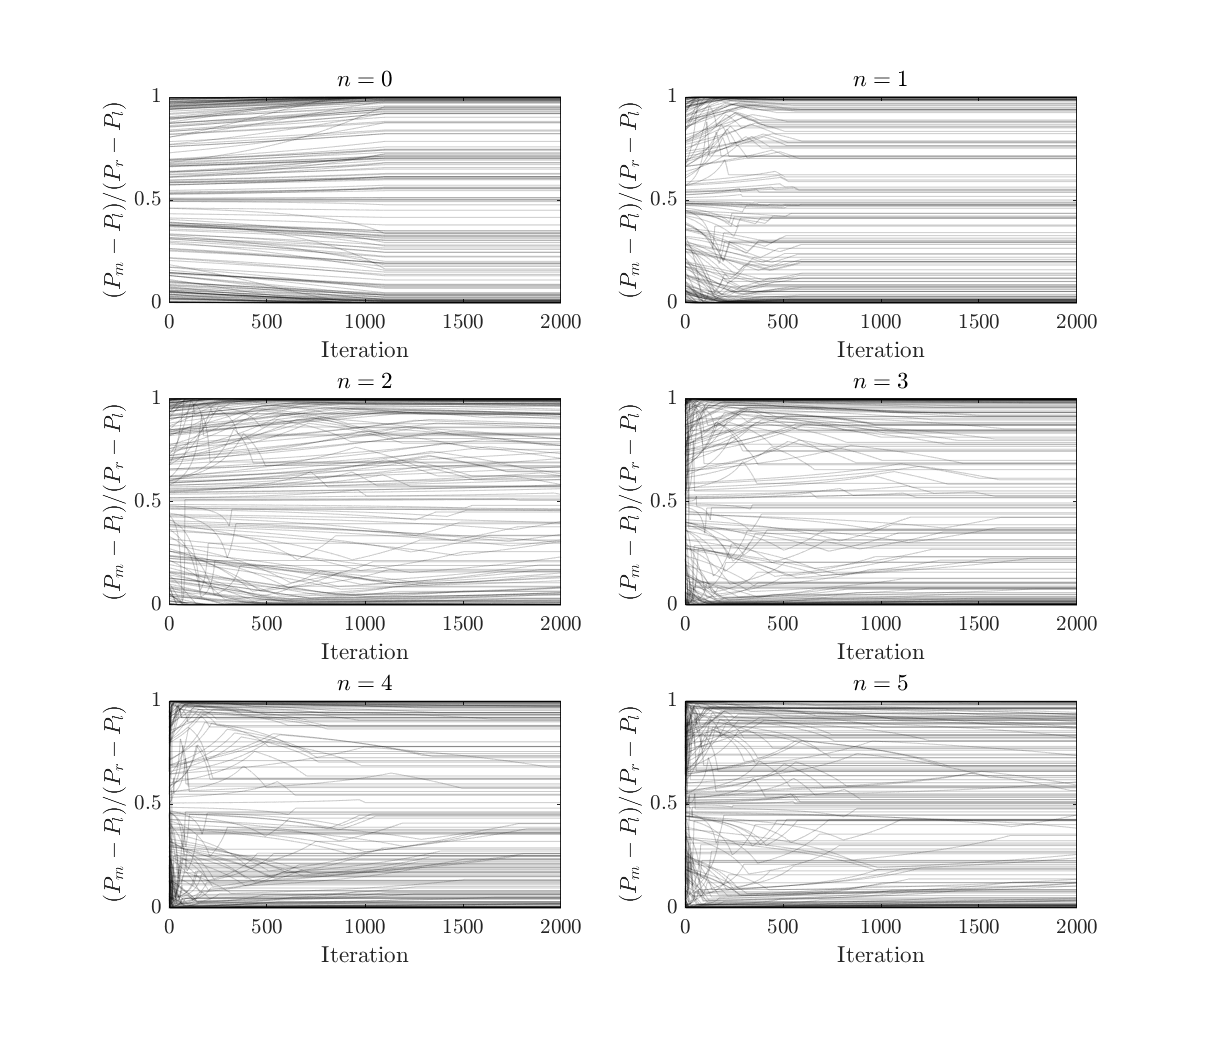
\includegraphics[width=1\textwidth]{./Figs/toy-model-series-clog}}
  \caption{Toy model for two pipes in series. In each iteration, we
    change the radius of the pipe as
    $r_{\text{new}} = r_{\text{old}} - \alpha
    Q_{i}/r_{\text{old}}^n$. Note that we set a maximum change of
    $\Delta r = \min{1,r}$.}
\label{toy-series-clog}
\end{figure}  



\subsubsection*{Parallel}
%
We also study the behavior when the pipes are in parallel (See
Fig. \ref{figure:resistor-par-clogging}). The numerical results of the
simulations are shown in Fig. \ref{toy-par-clog}. The behavior is
again very similar to the two pipes in series. We again find a similar
trend where the ratio of the $Q$'s remains unchanged. 
%
\begin{figure}[H]
  \begin{center}
    \begin{circuitikz}
      \draw
      (-0.5,0) node[anchor=east] {$P_{l}$} to [short] (0.1,0)
      -- (0.1,0.5) 
       to[R=$1/C_1$] (2,0.5)  -- (2,0) to [short] (2.5,0) node
       [anchor=west] {$P_r$};
      \draw
      (0.1,0)  --(0.1,-0.5) 
       to[R=$1/C_2$] (2,-0.5)  -- (2,0);
    \end{circuitikz} 
    \caption{Two resistors parallel together} \label{figure:resistor-par-clogging}
  \end{center}
\end{figure}


%
\begin{figure}[H]
  \centerline{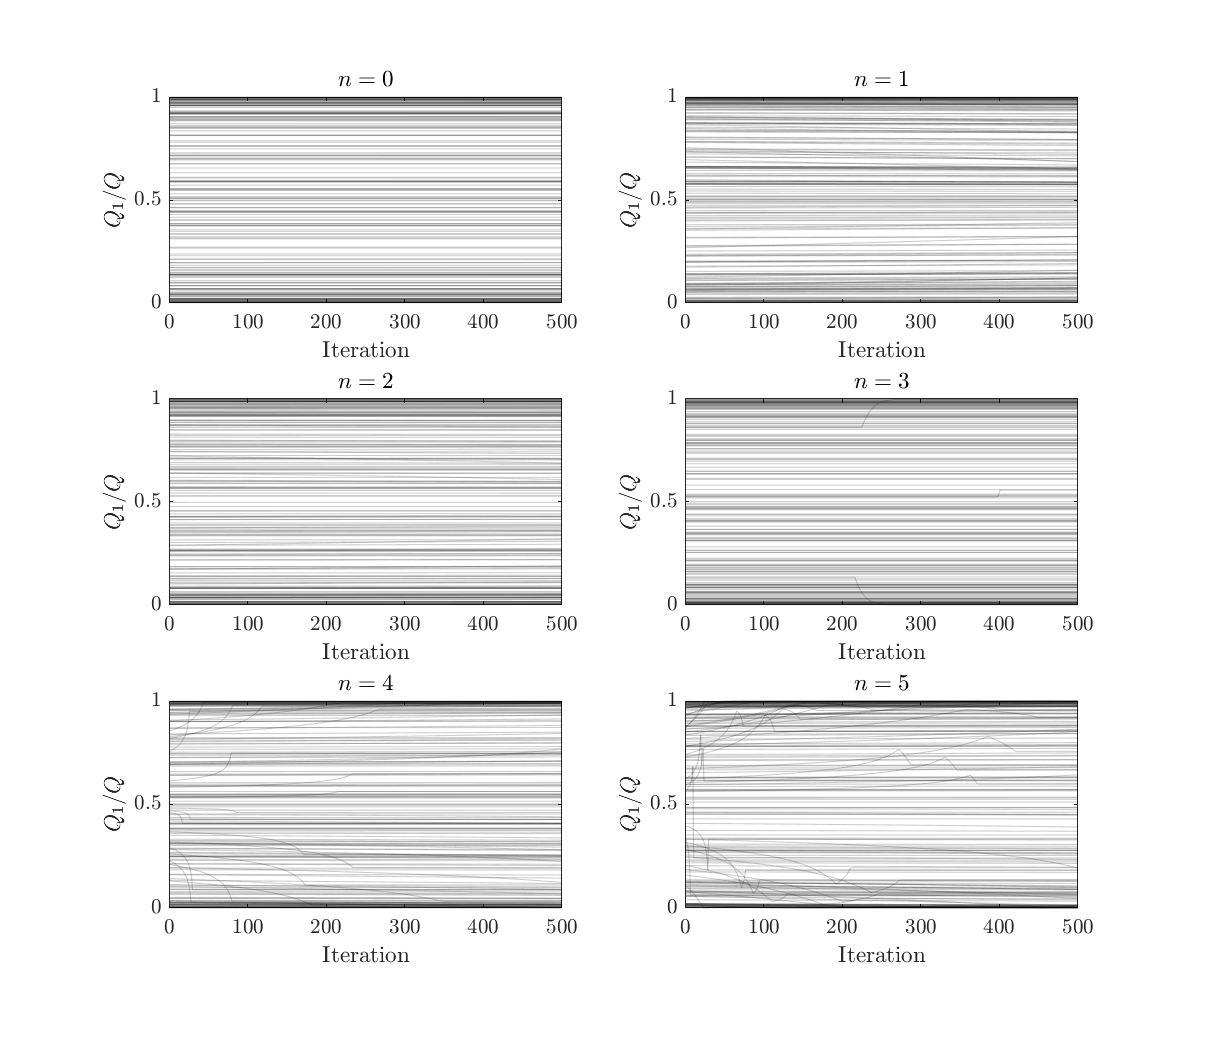
\includegraphics[width=1\textwidth]{./Figs/toy-model-par-clog}}
  \caption{Toy model for two pipes in series. In each iteration, we
    change the radius of the pipe as
    $r_{\text{new}} = r_{\text{old}} - \alpha
    Q_{i}/r_{\text{old}}^n$. Note that we set a maximum change of
    $\Delta r = \min{1,r}$.}
\label{toy-par-clog}
\end{figure}  


\subsection{Generalization of Erosion Law(Deng)}
Here is a naive guess of how the exponent of erosion law can change the network topology. We can assume the erosion law  
\begin{align}
    C &= a r^m \\
    \frac{dr}{dt} &= \frac{b Q}{r^n},
\end{align}
where $a,b,m,n$ are some constants. It can be derived that it is equivalent to
\begin{equation}
    \frac{dC}{dt} \propto QC^{1-\frac{n+1}{m}}.
\end{equation}
Particularly in previous series/parallel cases, $m=4$ and $n$ varies. We observed that $n<3$ leads to channeling while $n>3$ leads to homogeneity. Therefore, a reasonable guess is with the erosion law 
\begin{equation}
    \frac{dC}{dt} \propto Q^\alpha C^\beta,
\end{equation}
when $\alpha = 1$, the sign of $\beta$ will determine the channeling behavior. And the simulations as shown in Fig. \ref{fig:erosionExp} confirm the guess. Furthermore, we can see the change of flow distribution in terms of $P(Q)$, the distribution of flow in every resistor, as shown in Fig \ref{fig:PQ}. The exponential tail remains in the simulations for the $\beta = 0$ case. We do not have a theoretical explanation why the exponential tail remains in the $\beta = 0$ case.
\begin{figure}[H]
  \centerline{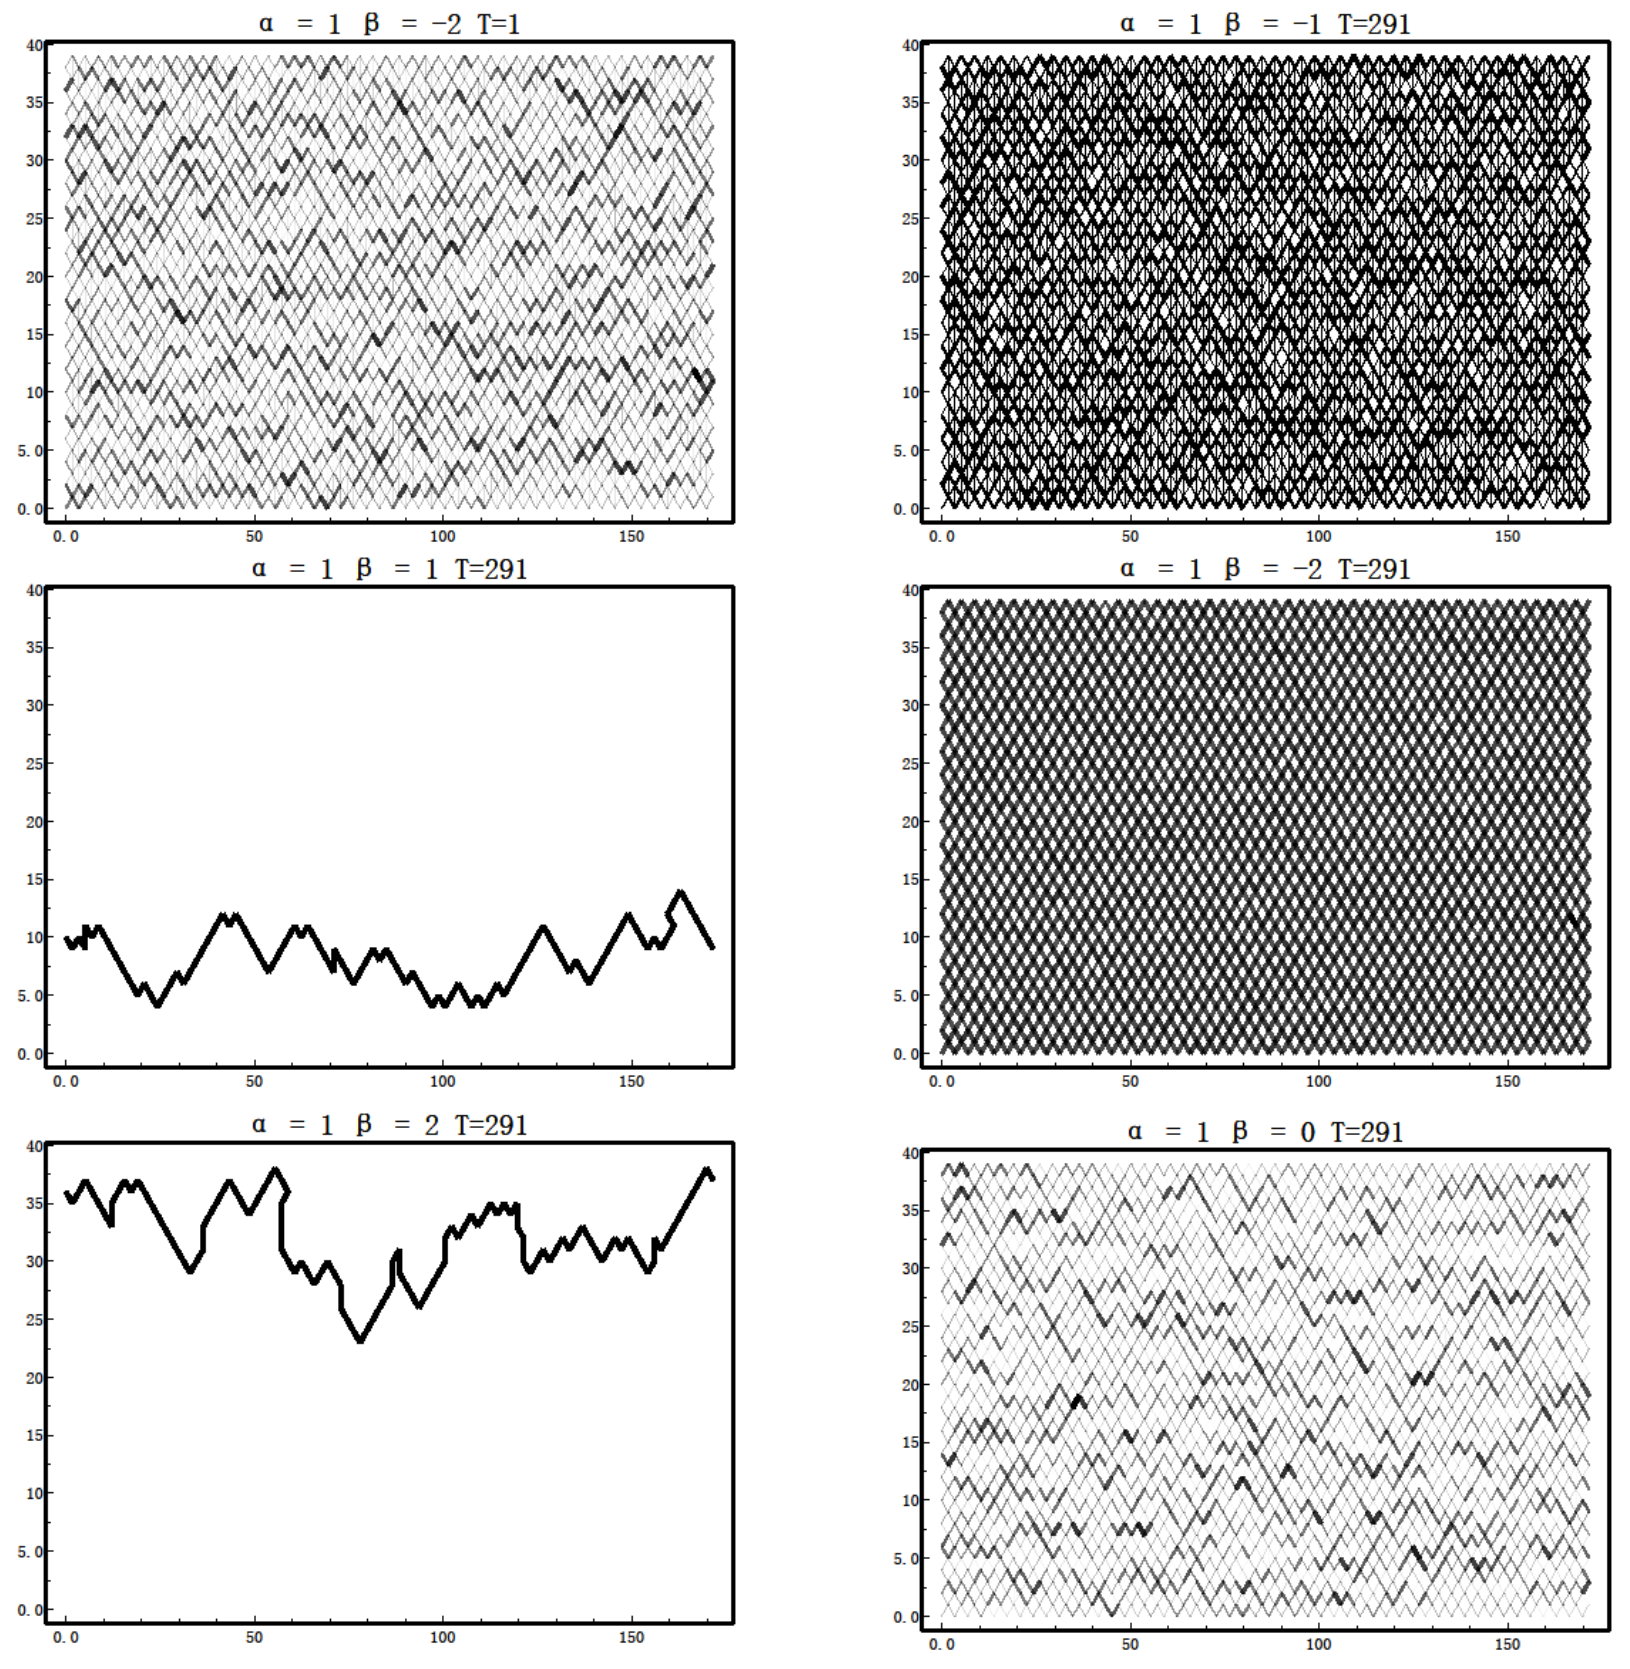
\includegraphics[width=1\textwidth]{./Figs/erosionExp.png}}
  \caption{A grid network erosion simulations with different $\beta$ exponents. Top left is the initial flow distribution for every simulation (T=1) and the rest are final distributions of the flow. We can easily distinguish the channeling ($\beta>0$) and homogenization behavior ($\beta<0$) from the results. }
\label{fig:erosionExp}
\end{figure}  

\begin{figure}[H]
    \centering
    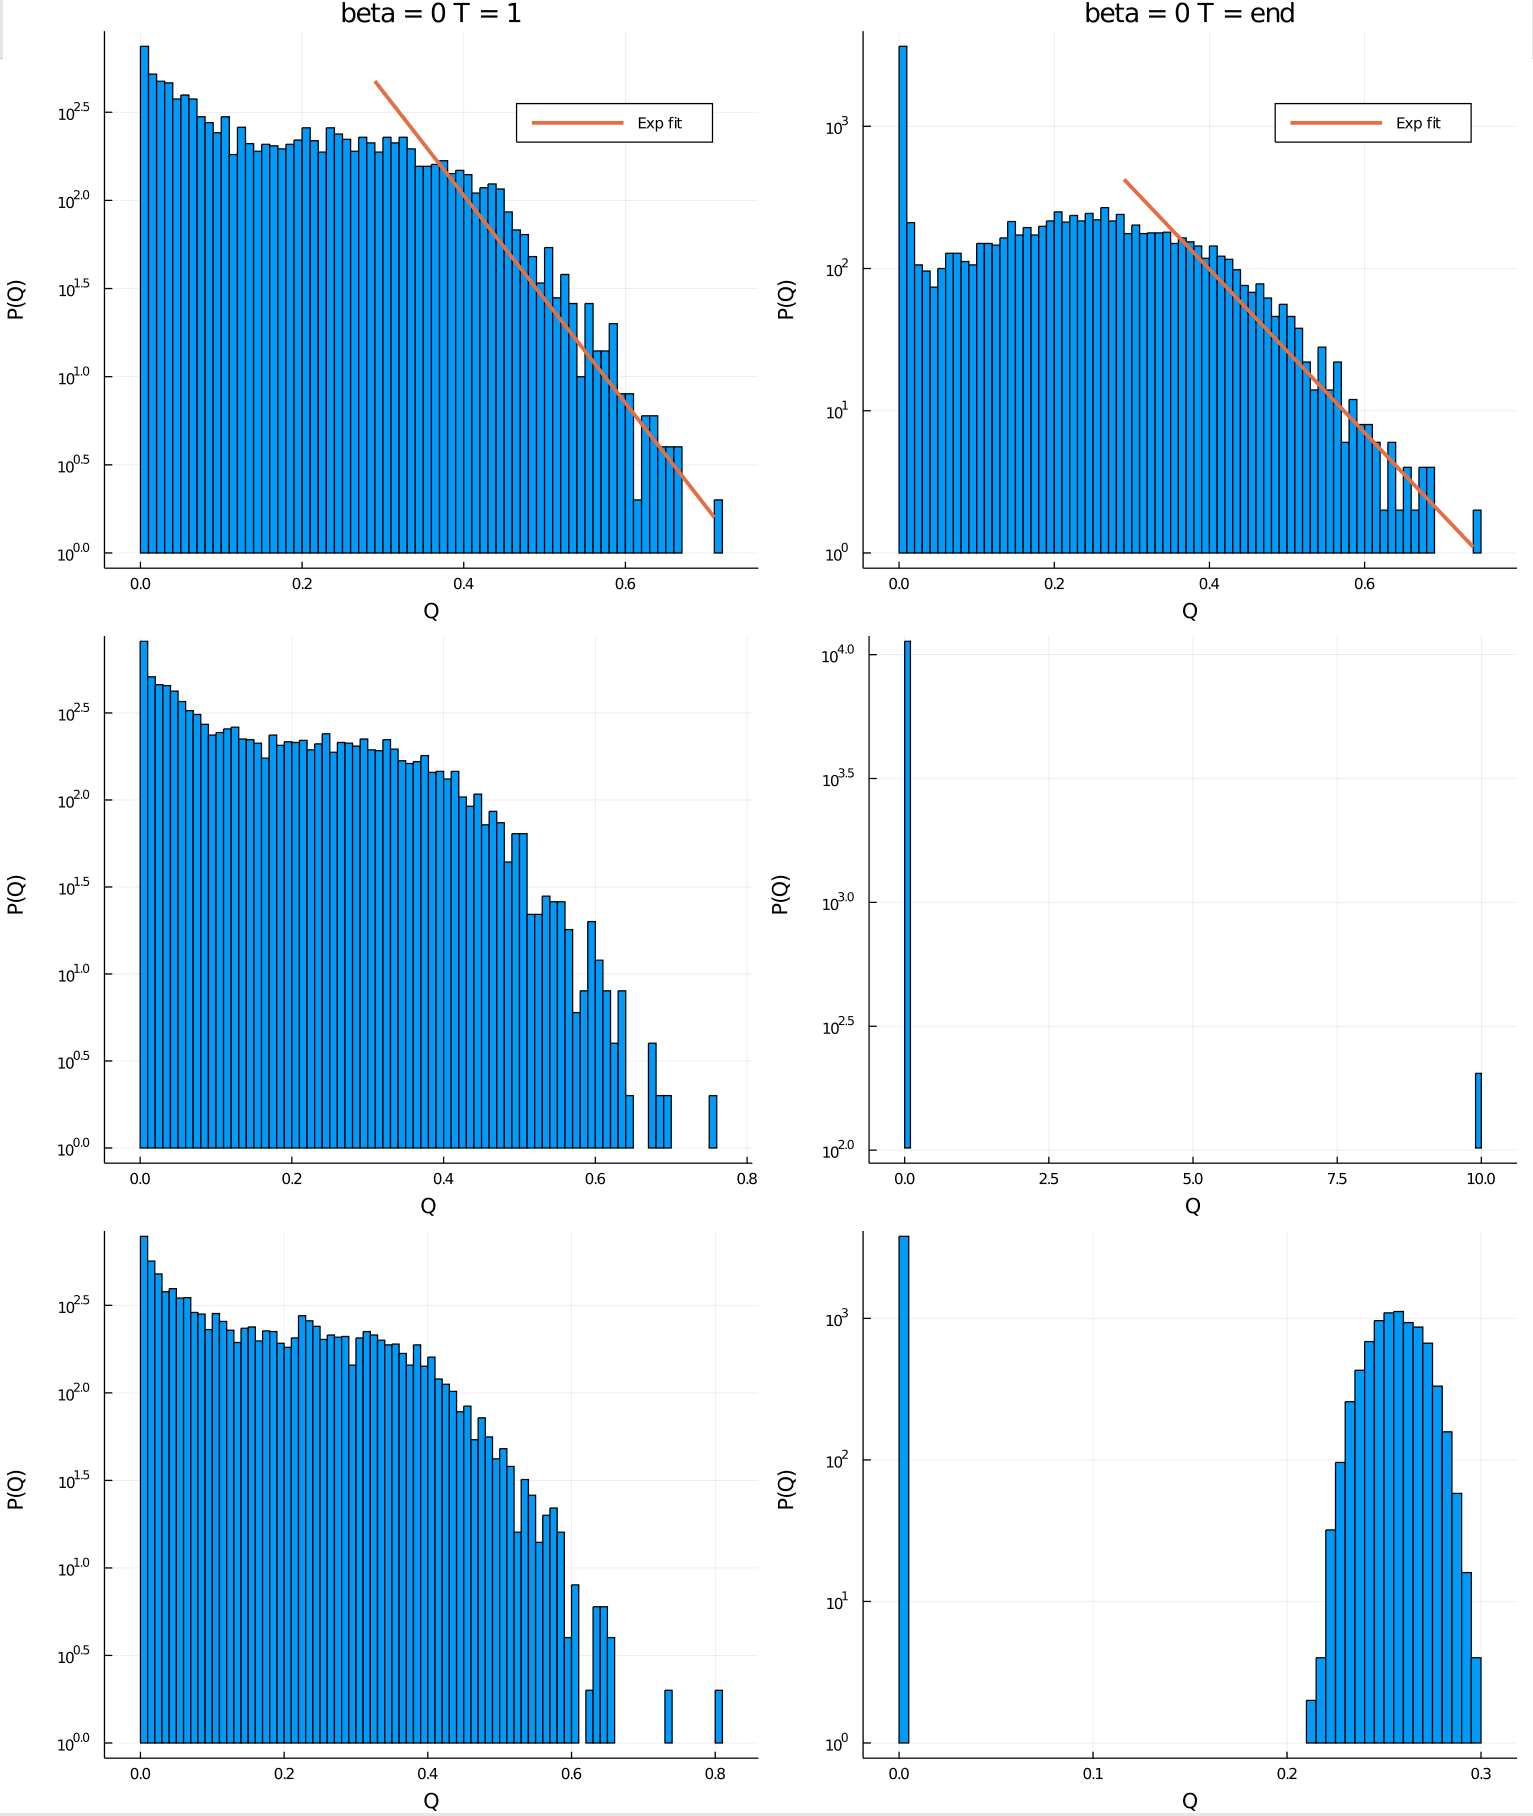
\includegraphics[width = 0.8\textwidth]{Figs/PQ.png}
    \caption{The flow distribution of networks in Fig \ref{fig:erosionExp} for different $\beta$'s. It is easy to distinguish channeling ($\beta = 1$), homogeneity ($\beta = -1$) and exponential tail ($\beta = 0$) from the flow distributions at the end of simulations. The delta function at $0$ is due to the resistors connecting vertically, which are perpendicular to the average flow.}
    \label{fig:PQ}
\end{figure}





\newpage

\section{Permeability modification model}
%
All the models introduced above represent different scenarios where
the clogging/erosion might happen. The question, however remains that
what could be a microscopic model? What it can predicts? and is there
a proxy (bulk property) that can be observed to study the microscopic
model?


We propose the following microscopic model: The polymers passing through pores are dragged by the flow. There are
two forces competing when a polymer adheres to the surface of a pore
(1) The drag force on the particle coming from flow, and (2)
ionic/VanderWaals or whatever force that tries to adhere the particles
to the surface. A particle attaches to the surface if the drag force
exerted by the fluid flow around it is smaller than the
VanderWaals/ionic force.

For simplicity, I assume that the force is ionic with a force distance
profile of $F= K/X^2$, where $K$ is a constant and $X$ is the
distance. I assume that polymers have an effective radius of $d_{p}$
and fluid viscosity is $\mu$ and the flow rate is $Q$. This model
states that the particle attaches to the surface when
%%
\begin{align}
    F_{\text{drag}} &\leq F_{\text{ionic}}\\
    6\pi \mu d_{p} \frac{2Q}{\pi R^2} \lp 1- \frac{r^2}{R^2} \rp & \leq \frac{K}{(R-r)^2} \\
    1 - \frac{r^2}{R^2} & \leq \lp \frac{K }{12 \mu  d_{p} Q} \rp \frac{1}{\lp 1 - r/R \rp^2} \\
    1 & \leq \frac{r^2}{R^2} + \alpha \frac{1}{\lp 1-r/R\rp ^2}
\end{align}
%
where $\alpha = K/\lp 12\mu d_pQ \rp$ is a factor that compares the ionic force and viscous
force. Note that it depends on the flux rate. If we define
$x = 1- r/R$ we obtain
%
\begin{align}
    1 &\leq (1-x)^{2} + \frac{\alpha}{x^2} \\
    x^2- x^2(1-x)^{2} &\leq \alpha \\
    x^2 (1- (1-x)^2) & \leq \alpha \\
    x^3(2-x) & \leq \alpha \\
    \text{if } x\ll1 \to x & \leq \lp \frac{\alpha}{2}\rp^{1/3}
\end{align}
%
%
\begin{figure}[H]
  \centering
  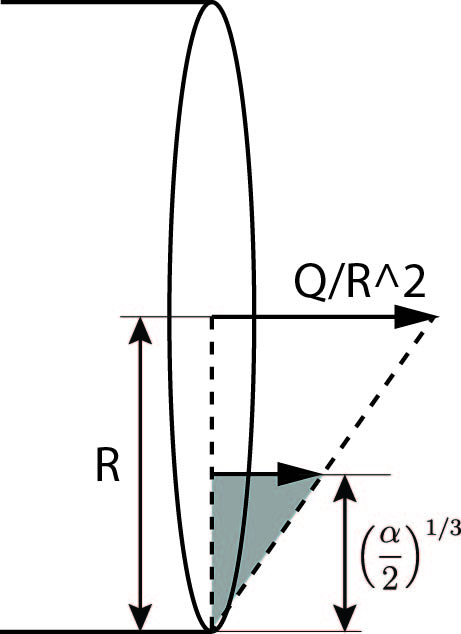
\includegraphics[width=4cm]{./Figs/model2.jpg}
  \caption{Flow in the pipe}
\end{figure}
%
As a result the distance is proportional to $\alpha^{1/3}$. Note that
$\alpha$ depends on $1/Q$.  Now, lets
find the flux passing through this adsorption layer (any polymer in
this layer would attach to the surface)
%
%
\begin{align}
  \text{volume}/\text{time} &= \frac{1}{2} R \alpha ^{1/3} \cdot \frac{Q}{R^{3}} R\a^{1/3} \cdot 2\pi R = \pi Q \a^{2/3}  = \pi \lp \frac{K  }{12 \mu  d_{p}} \rp^{2/3} Q^{1/3} \\
  \text{volume}/\text{time} & \propto {Q^{1/3}} 
\end{align}
%
Now, if we assume that the number of polymers passing through the area
cause clogging of the pipe and change the total area of the pipe, then
we find that

%
\begin{align}
  d (\pi R^2) \propto Q^{1/3} \quad \to \quad R dR \propto Q^{1/3}
\end{align}
%
We also know that $k = \pi R^4/8l^2$, as a result
%
\begin{align}
  dk \propto R^{3} dR \\
  dk \propto R^2 Q^{1/3} \\
  dk \propto Q^{1/3}
\end{align}

\subsection*{Experimental Results}
%
In Shima's paper, we report a figure that shows the evolution of
permeability $k$ per volume of polymer $V_{pol}$ that passes through
the porous media. Basically we are plotting $\Delta k$ versus $Q$
passing through the porous media. The figure and best polynomial fit
is shown blow
%
%
\begin{figure}[H]
  \centering
  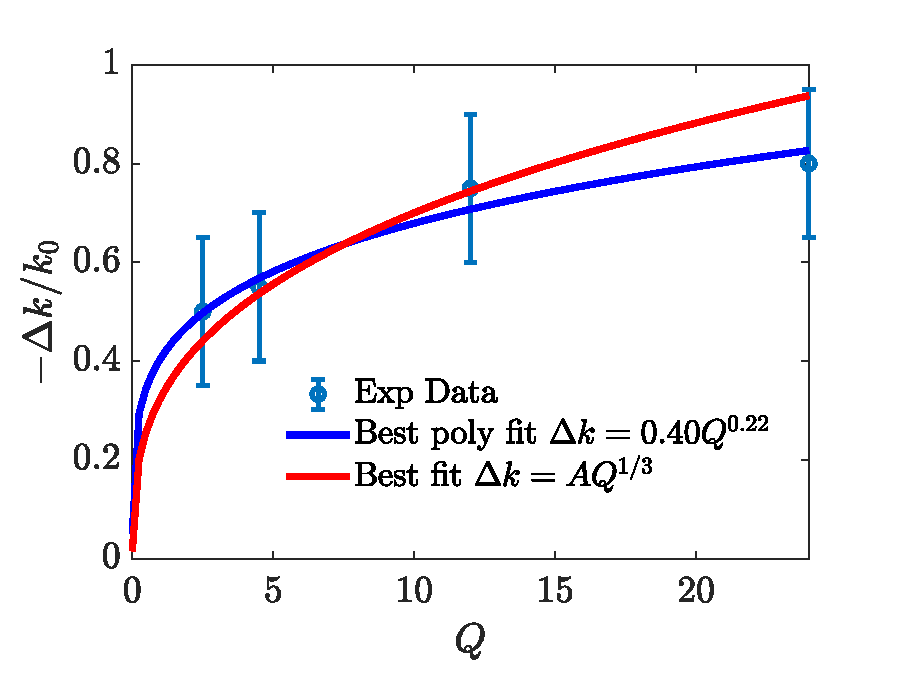
\includegraphics[width=0.55\textwidth]{./Figs/k-evolution.eps}
  \caption{$k$ versus volume of fluid passed through a porous media}
\end{figure}


\section{Foam Relaxation and Non-monotonic Aging}
%
So far the observation is that no matter how much disorder we
introduce in the size distribution of pipe diameters, no relaxation
behavior can be observed in a structured random network of tubes. If
we prune the network, near the percolation limit, the slow $log(t)$
dynamics is observable, however, it seems to be very unlikely that it
is the case. We need to introduce a toy model that can capture this
behavior. My intuition is that the relaxation is due to aging of the
adhesion of pore surfaces attaching to each other due to compression.
%


\subsection{Modeling}
%
We assume a network of pores, as we did before. The network of the pores are shown in Fig. \ref{fig:relaxation-network}. The pores are with different size. the connections are also with different sizes. 
%
\begin{figure}[H]
  \centering
  % 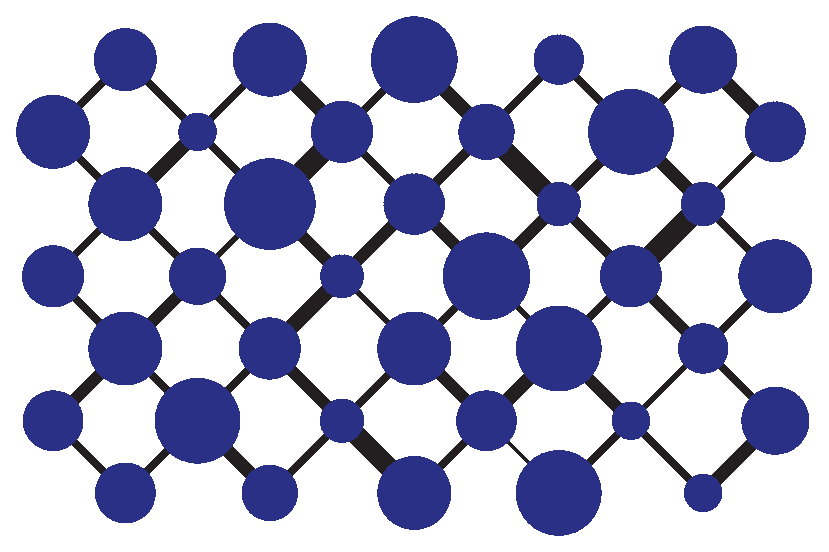
\includegraphics[width=0.55\textwidth]{./Figs/relaxation_grid}
  \caption{An example of pores connected with different sizes and different resistors} \label{fig:relaxation-network}
\end{figure}
%
On a structured grid, we initialize a random distribution of pore sizes, with random resistor connections. For each pore, we have a four neighbors. We first  need to determine the initial pressure of the pores. \red{I don't have a good way to initialize the pressures, for now, I consider them to be the same amount. It could also depend on the initial volume.} Due to Darcy's law we have
%
\begin{align}
    Q_{ij} = \frac{\pi r_{ij}^4}{8 \mu L_{ij}} \left( {P_i - P_j}\right) = \frac{P_i - P_j}{R_{ij}}, \qquad R_{ij} \equiv \frac{8 \mu L_{ij}}{\pi r_{ij}^4}
\end{align}
%
Where $r_{ij}$ and $L_{ij}$ are radius and length of the resistors connecting the pores. $Q_{ij}$ represents the outflux from node $i$ to node $j$. At each time for each pore, we can calculate the total out-flux of the flow is as 
%
\begin{align}
    Q_i = \sum_{j \in N(i)} Q_ij = \sum_{j \in N(i)} \frac{\pi r_{ij}^4}{8 \mu L_{ij}} \left( {P_i - P_j}\right)
\end{align}
%
where $N(i)$ represents the neighbors of $i$-th node. After calculating the total outflux, we need to find an equation on how to update the pressure of the pore $P_i$. If we assume that ideal gas law, we have
%
\begin{align}
    P_i V_i = m_i RT \quad \dot{m_i} = - \rho Q_i \quad \text{(minus sign is since } Q_i \text{ is out-flux)} 
    \end{align}
%
Assuming a constant density, we have
%
\begin{align}
    \frac{d P_i}{dt} = \frac{RT}{V_i} \frac{d m_i}{dt}  = -\frac{\rho RT}{V_i} Q_i \\
    \frac{d P_i}{dt} = - \frac{\rho RT}{V_i} \sum_{j \in N(i)} \frac{P_i - P_j}{R_{ij}}  
\end{align}
%
In the matrix format this can be written as 
%
\begin{align}
\frac{d\mathbf{P}}{dt} = \mathbf{D} \cdot \mathbf{A} \cdot \mathbf{P}\\
\mathbf{P} = \begin{bmatrix} P_1 \\ \vdots \\ P_n
\end{bmatrix}\\
\mathbf{D} = \text{diag}(\frac{-\rho R T}{V_1},\cdots, \frac{-\rho R T}{V_n})\\
[\mathbf{A}]_{ij} = -\frac{1}{R_{ij}}, \quad [\mathbf{A}]_{ii} = \sum_{i\in N(i)} \frac{1}{R_{ij}}
\end{align}
%
To solve the above equations, we expand the LHS to obtain
%
\begin{align}
    \frac{d\mathbf{P}}{dt} = \mathbf{D} \cdot \mathbf{A} \cdot \mathbf{P} \\
    \frac{\mathbf{P}_{n+1}- \mathbf{P}_n}{\Delta t} = \mathbf{D} \cdot \mathbf{A} \cdot \left( \theta \mathbf{P}_{n+1} + (1-\theta) \mathbf{P}_{n}\right) \\    
    \left( \mathbf{I} - \theta\Delta t \mathbf{D}\mathbf{A} \right) \mathbf{P}_{n+1} = \left( \mathbf{I} + (1-\theta) \Delta t \mathbf{D} \mathbf{A}\right) \mathbf{P}_n
\end{align}
%
Note that $0 \leq \theta \leq 1$. Having $\theta = 0$, the solution becomes explicit forward Euler, and $\theta = 1$, the equations become implicit method. Note that for a given geometry $\mathbf{D}$ and $\mathbf{A}$ are fixed and the solution can be obtained through matrix multiplication as
%
\begin{align}
 \mathbf{P}_{n+1} = \left( \mathbf{I} - \theta\Delta t \mathbf{D}\mathbf{A} \right)^{-1} \left( \mathbf{I} + (1-\theta) \Delta t \mathbf{D} \mathbf{A}\right) \mathbf{P}_n
\end{align}
%
Using the above relations, I found that the relaxation does not happen over multiple decades. It seems very unlikely that the porous structure is causing this slow relaxation. 
\begin{figure}[H]
  \centering
  % 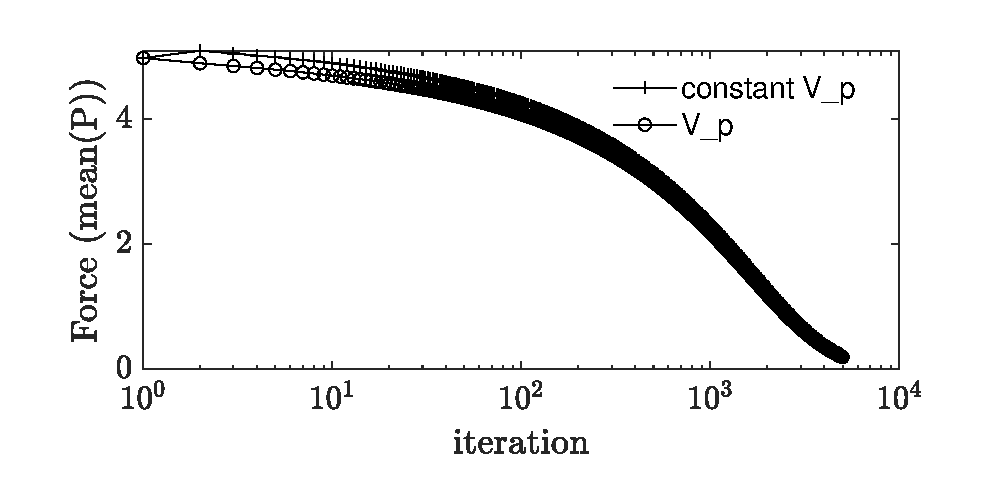
\includegraphics[width=0.55\textwidth]{./Figs/relaxation-porous.eps}
  \caption{Mean pressure relaxation in a random network of pores with a constant pore size and random pore size.} \label{relaxation}
\end{figure}

Looking at the microgrpah image of open-cell foams (as shown in Fig. \ref{micrograph}), it seems unlikely that the fluid is playing a role in this. 
%
\begin{figure}[H]
  \centering
  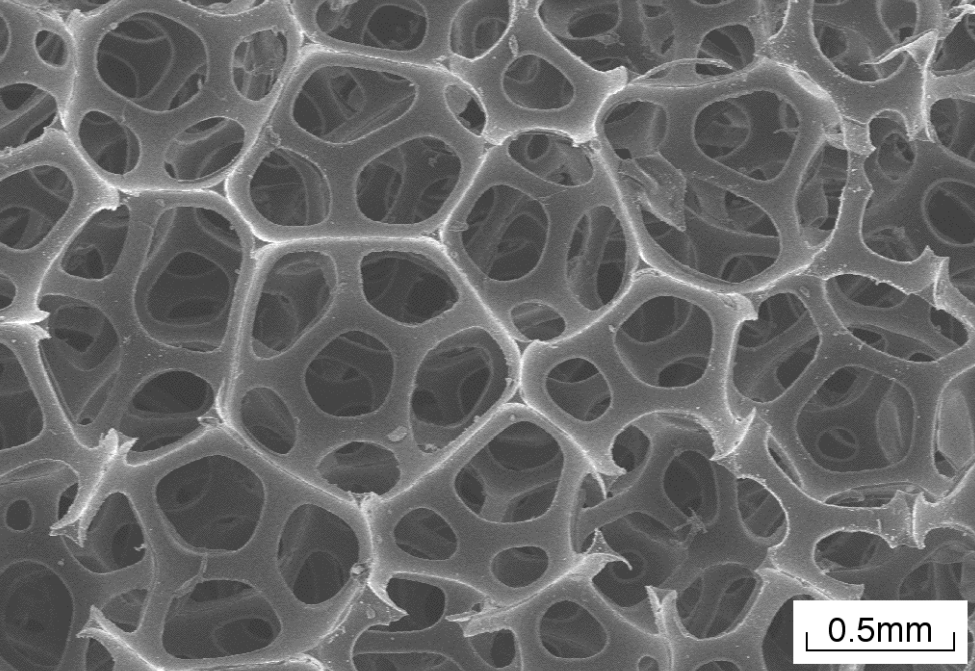
\includegraphics[width=0.45\textwidth]{./Figs/micrograph-open-cell.png}
  \caption{Micrograph showing cellular microstructure of a polyester urethane foam (100 ppi) (Taken from \cite{gong2005compressive}) } \label{micrograph}
\end{figure}
%
I believe that since the material is visco-elastic, the response is due to the polymer structure that have a large relaxation times. 








\section{Distribution of Resistor-level response}
%
We consider a random resistor network. In this network, we remove a single resistor, remove it from the network. The permeability changes. We then record the PDF of the change in permeability. 
The result looks as follows
%



\section{Flow-Chains: Force-Chains}
%
We observe patterns similar to force-chains observed in granular
materials, but in porous media. See Fig. \ref{flow-chain}. For a movie
of this behavior see
\href{https://www.youtube.com/watch?v=E8sVcxipNio}{this link}.

\begin{figure}[H]
  \centering
  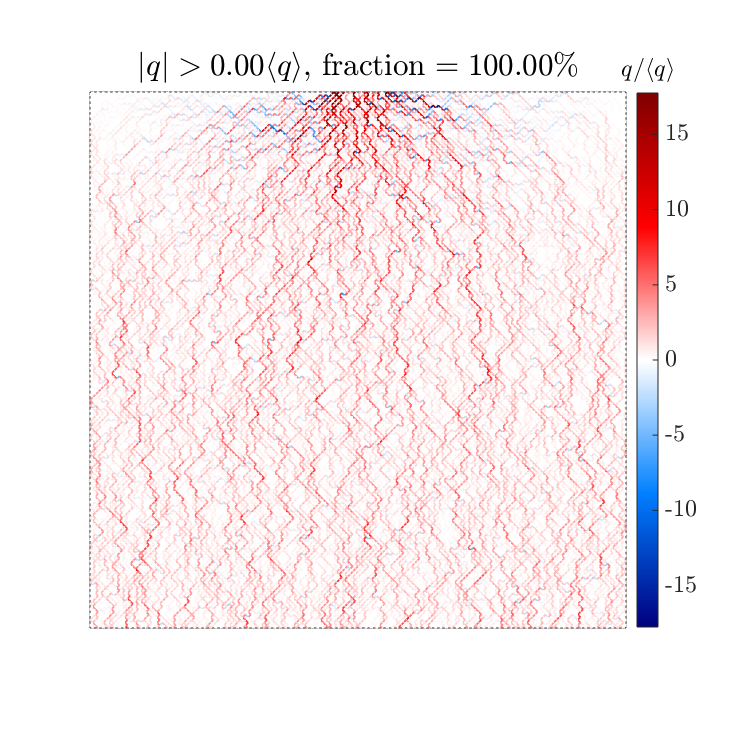
\includegraphics[width=0.45\textwidth]{./Figs/flowchain1}
  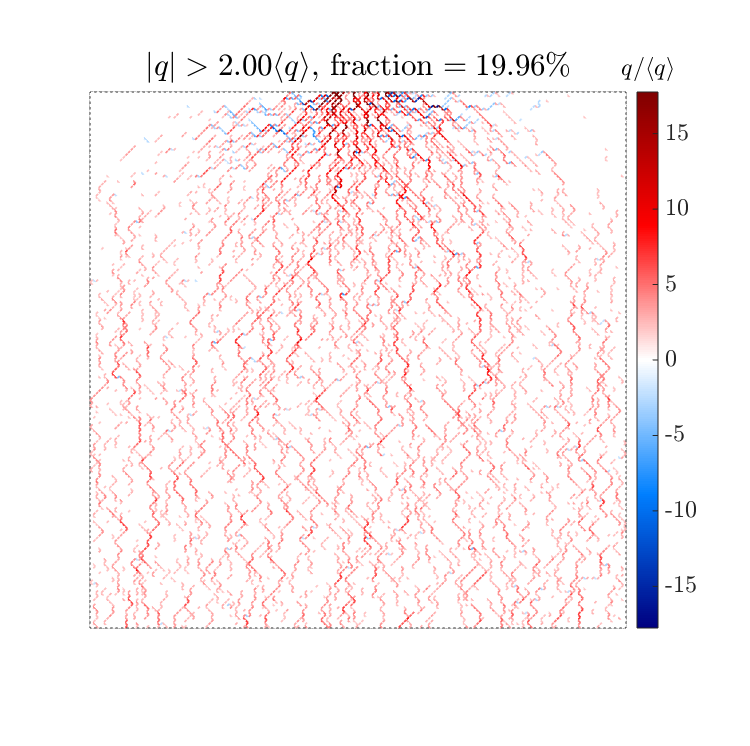
\includegraphics[width=0.45\textwidth]{./Figs/flowchain2}
  \caption{Force chain behavior in porous media.} \label{flow-chain}
\end{figure}





\end{document}

